\documentclass[letter,12pt]{article}
\usepackage{graphicx}
\begin{document}

% \begin{tabular}{5}{ccccc}
\noindent 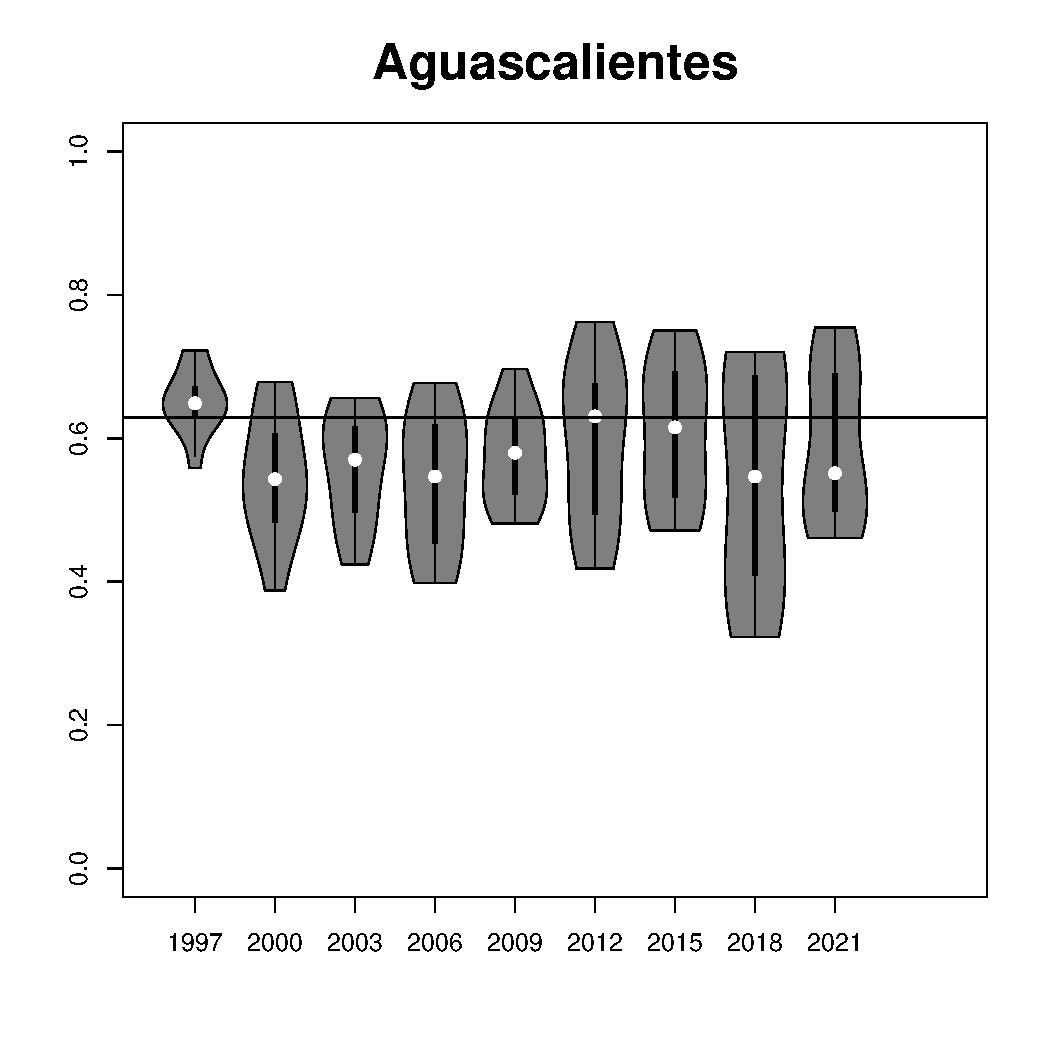
\includegraphics[width=.18\textwidth]{1.pdf}  
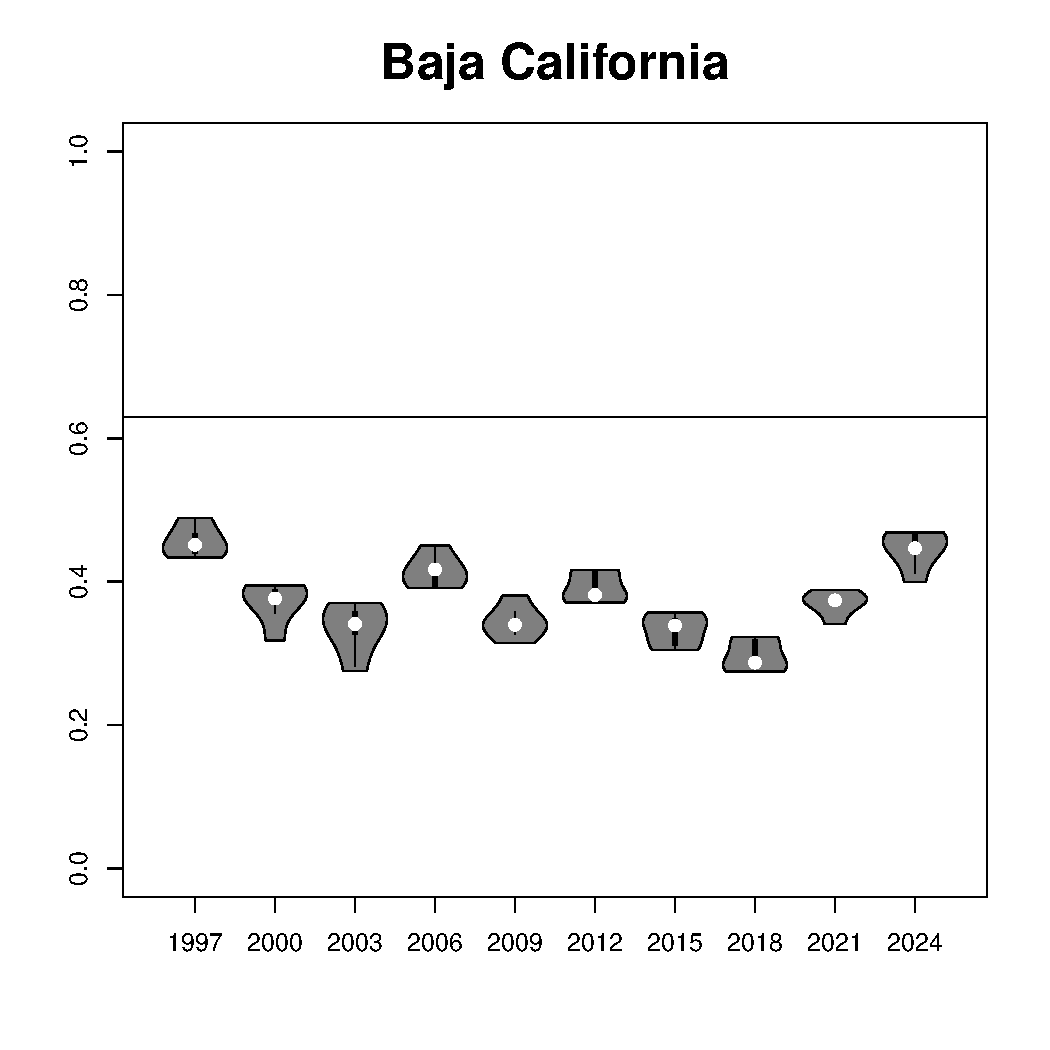
\includegraphics[width=.18\textwidth]{2.pdf}  %&
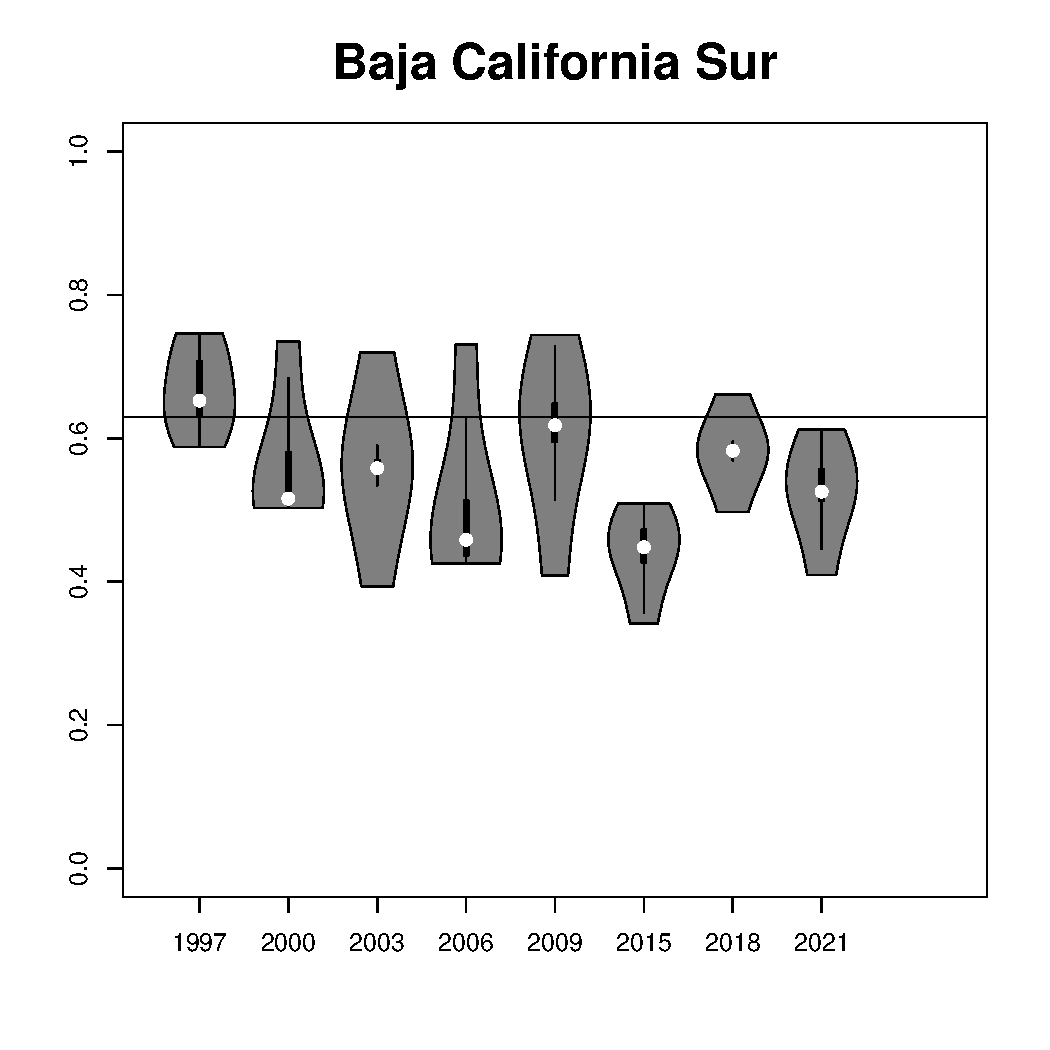
\includegraphics[width=.18\textwidth]{3.pdf}  %&
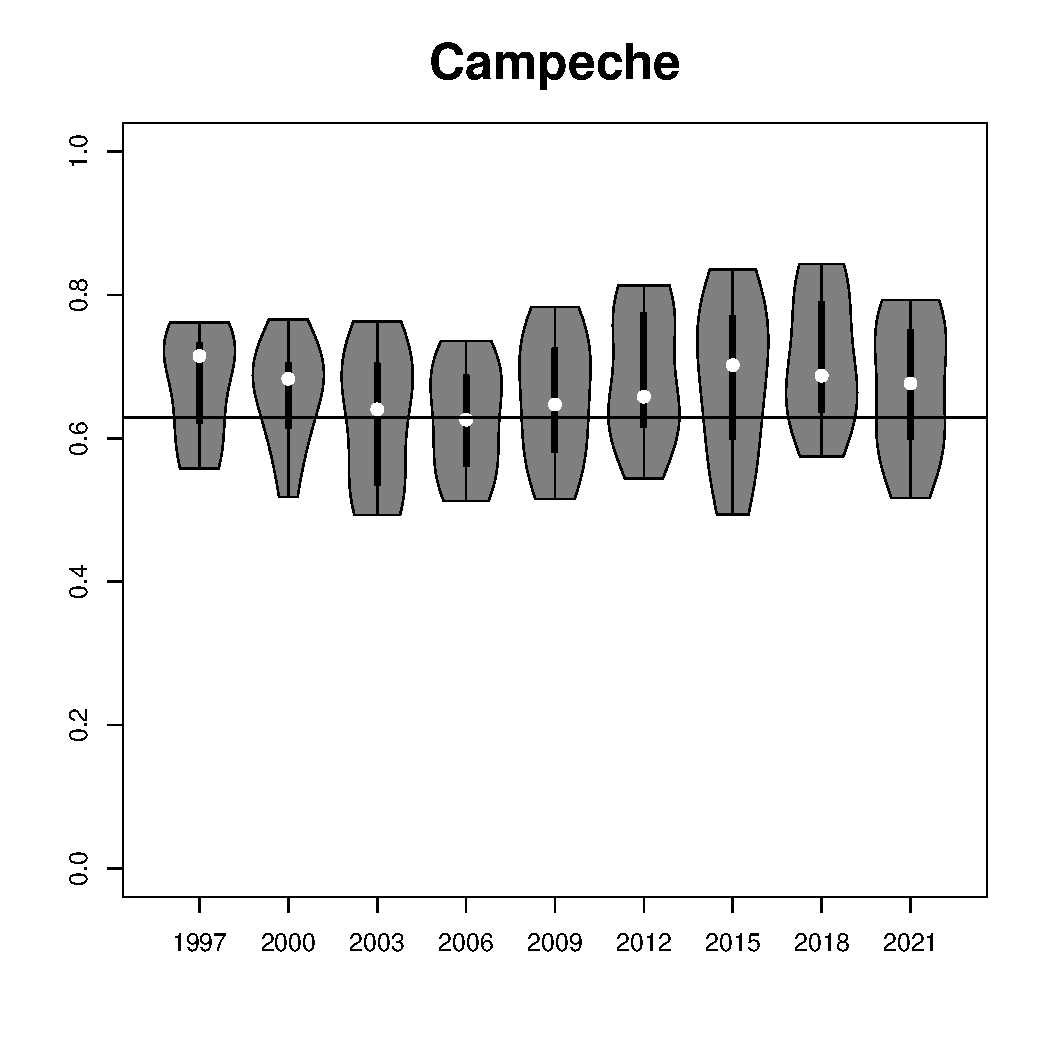
\includegraphics[width=.18\textwidth]{4.pdf}  %&
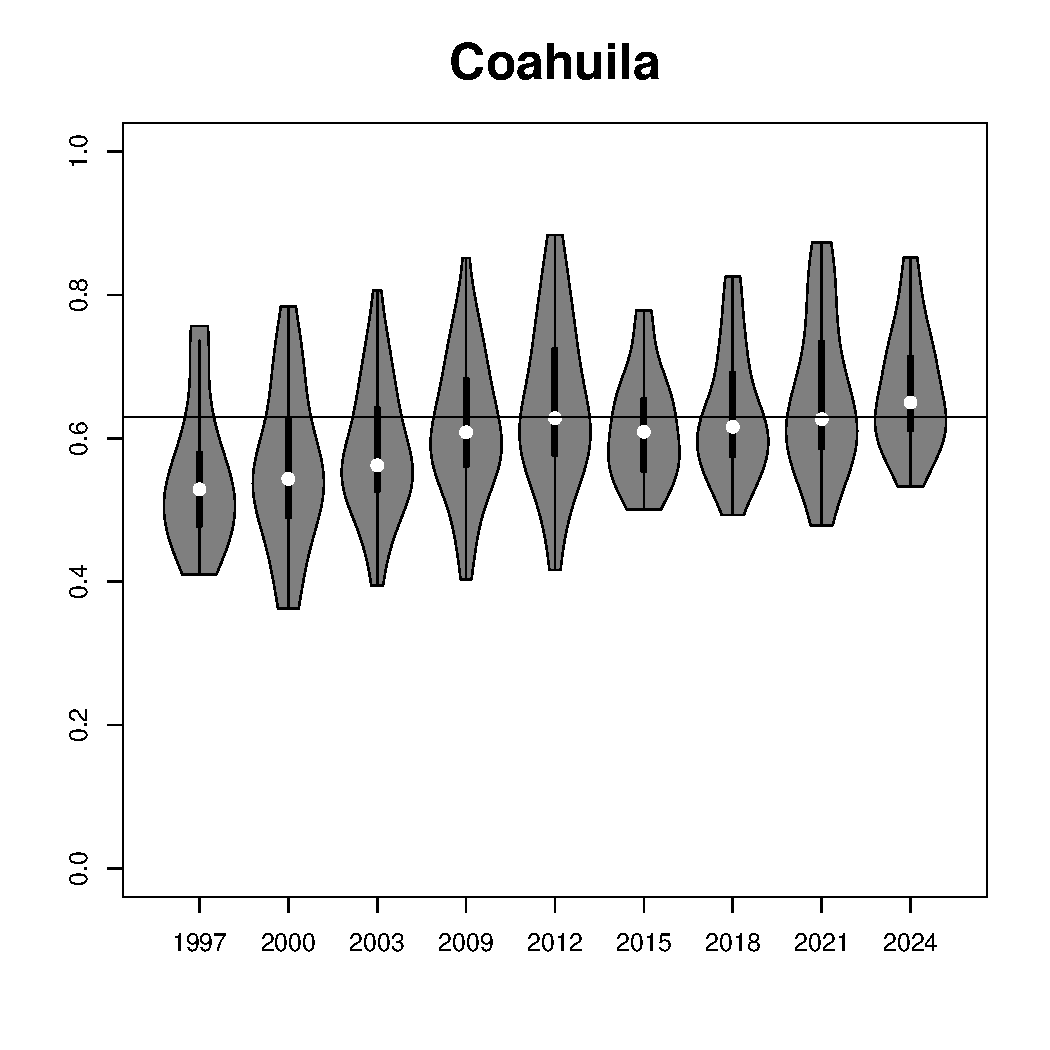
\includegraphics[width=.18\textwidth]{5.pdf}  %\\
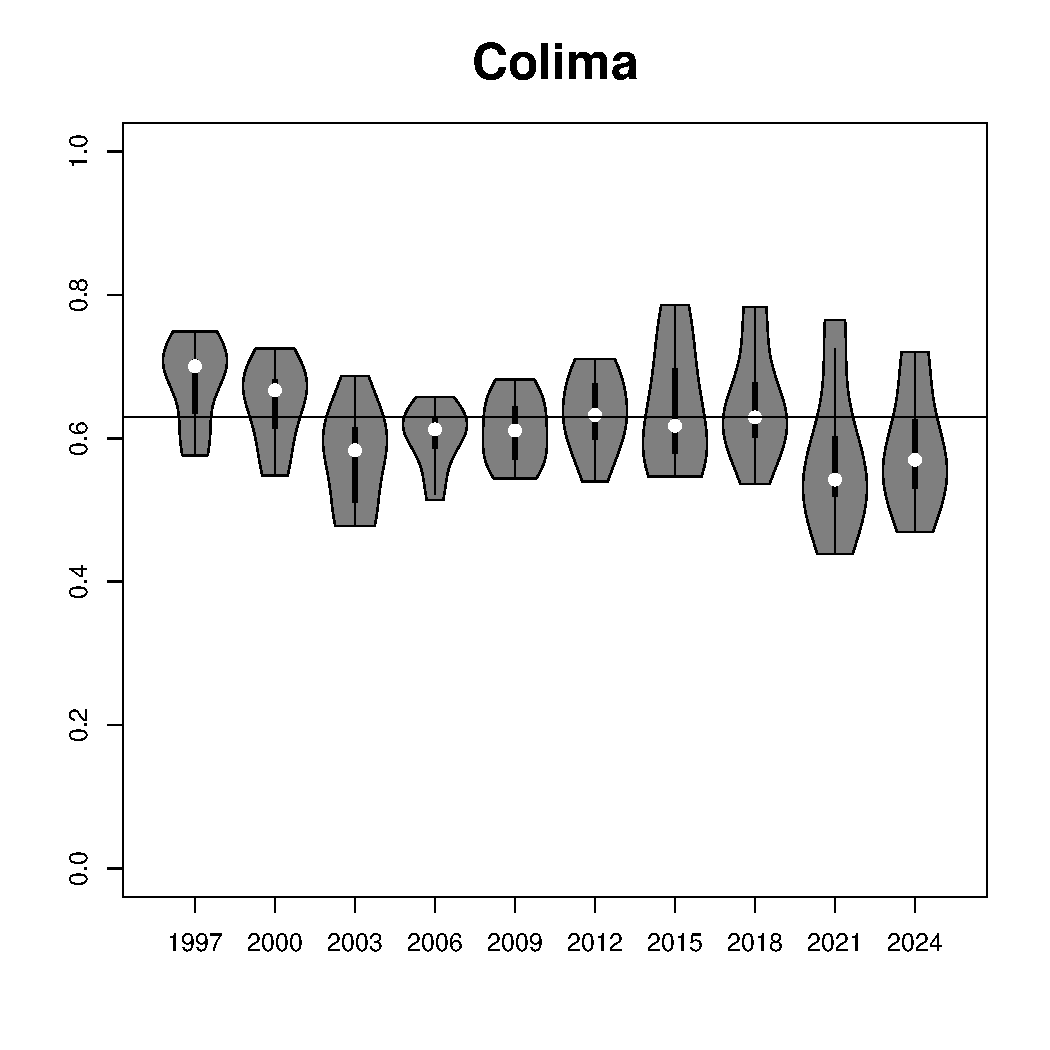
\includegraphics[width=.18\textwidth]{6.pdf}  %&
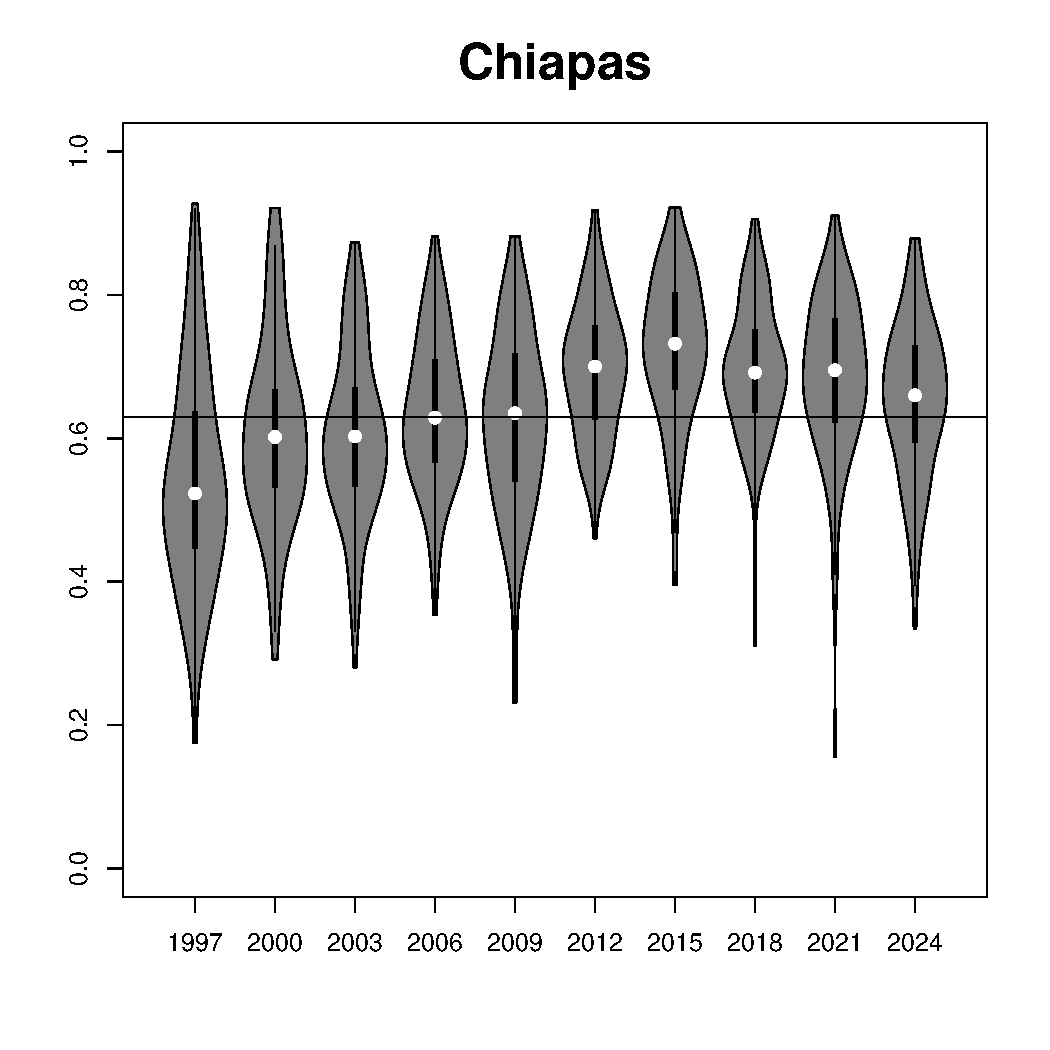
\includegraphics[width=.18\textwidth]{7.pdf}  %&
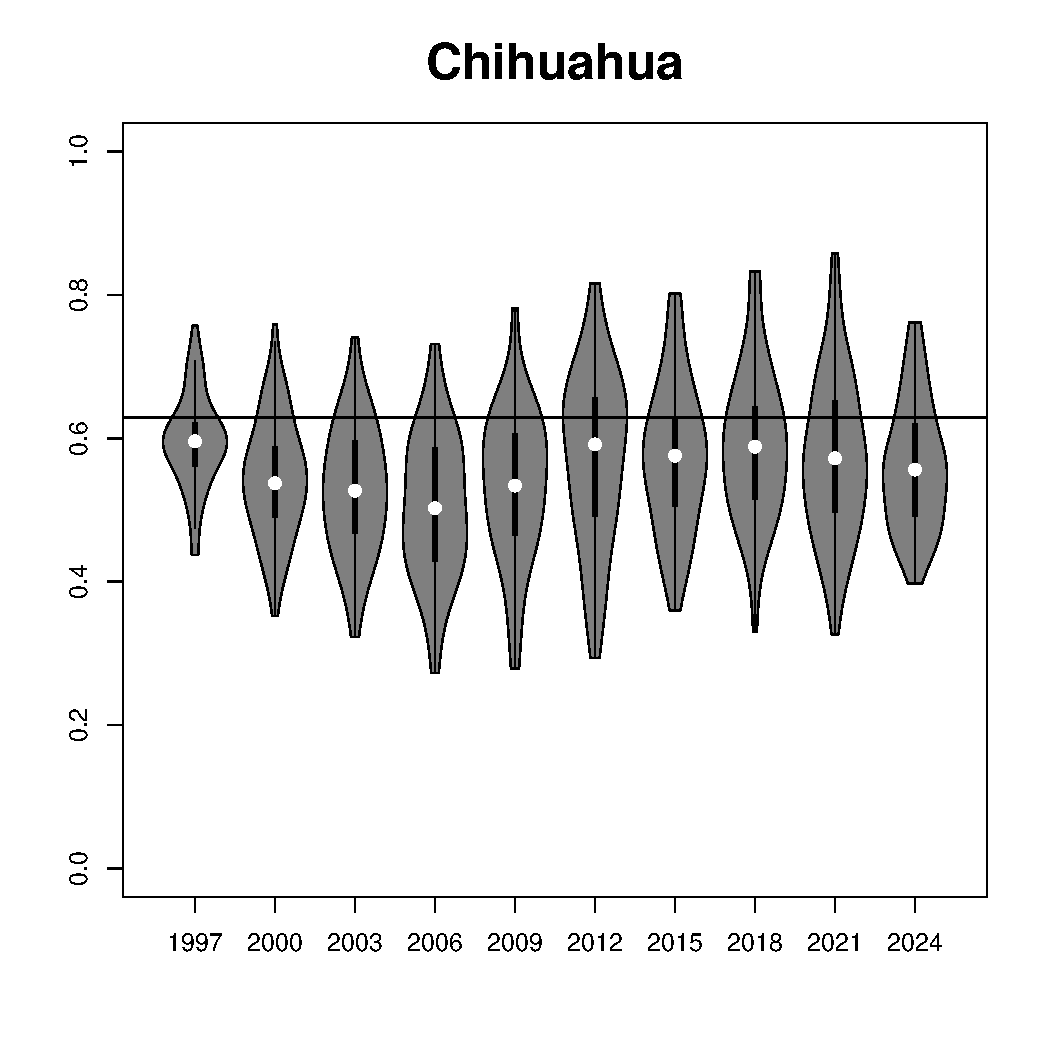
\includegraphics[width=.18\textwidth]{8.pdf}  %&
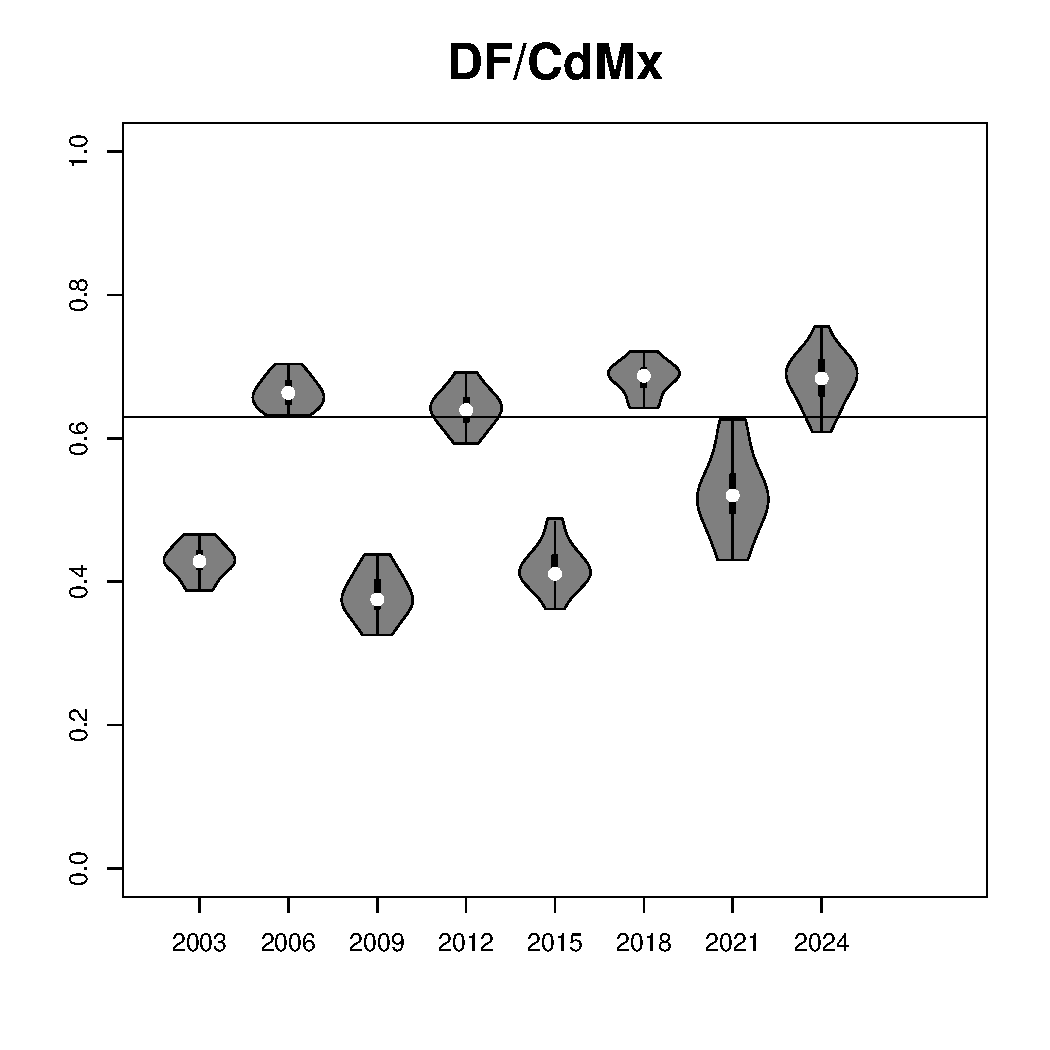
\includegraphics[width=.18\textwidth]{9.pdf}  %&
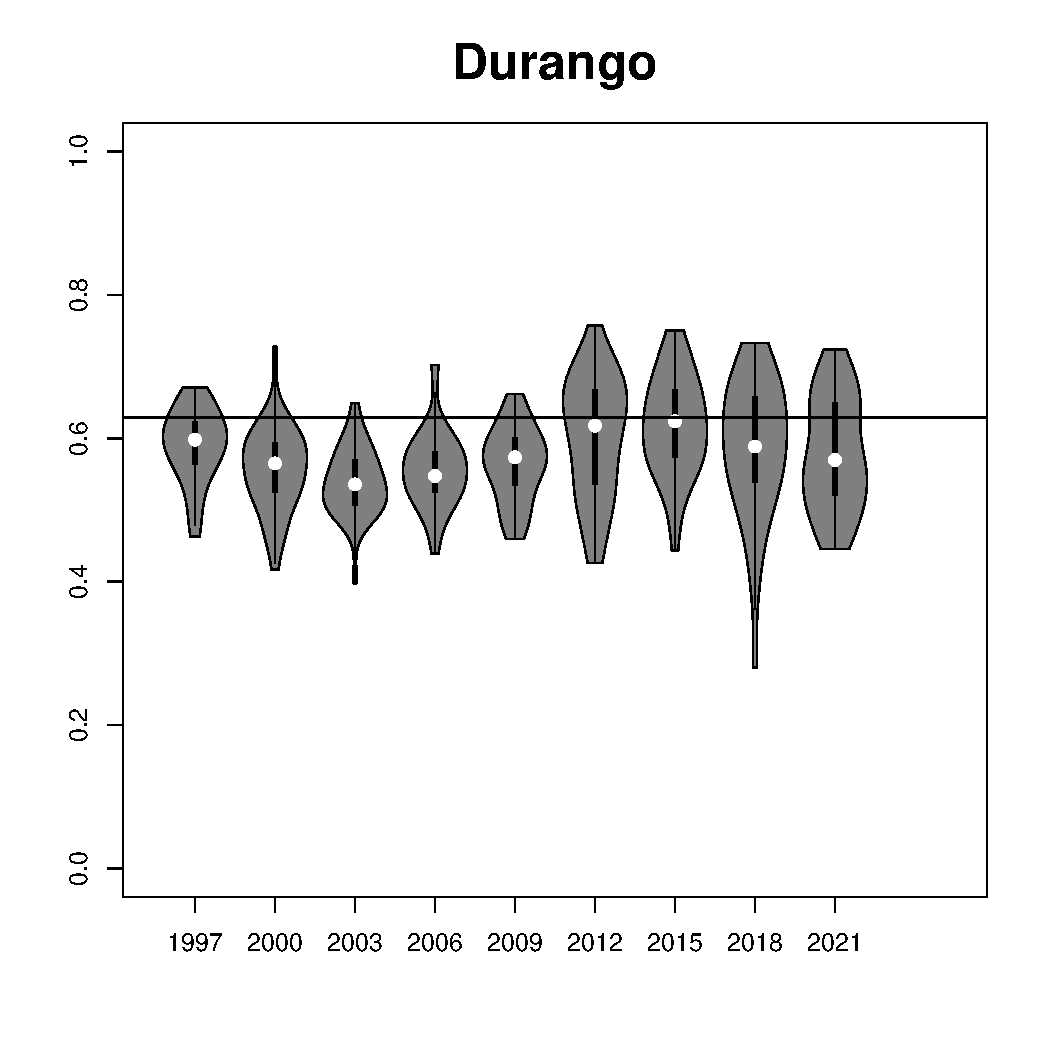
\includegraphics[width=.18\textwidth]{10.pdf} %\\
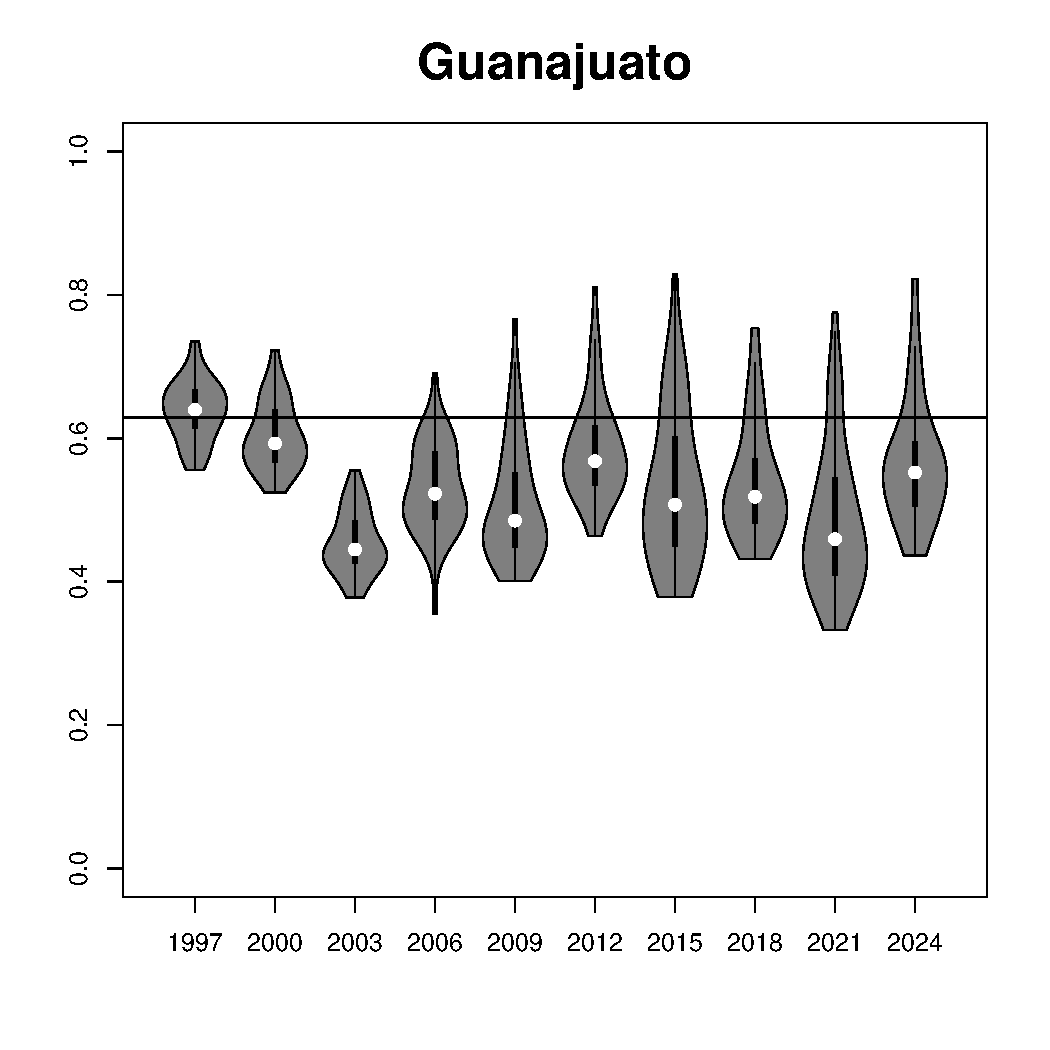
\includegraphics[width=.18\textwidth]{11.pdf} %&
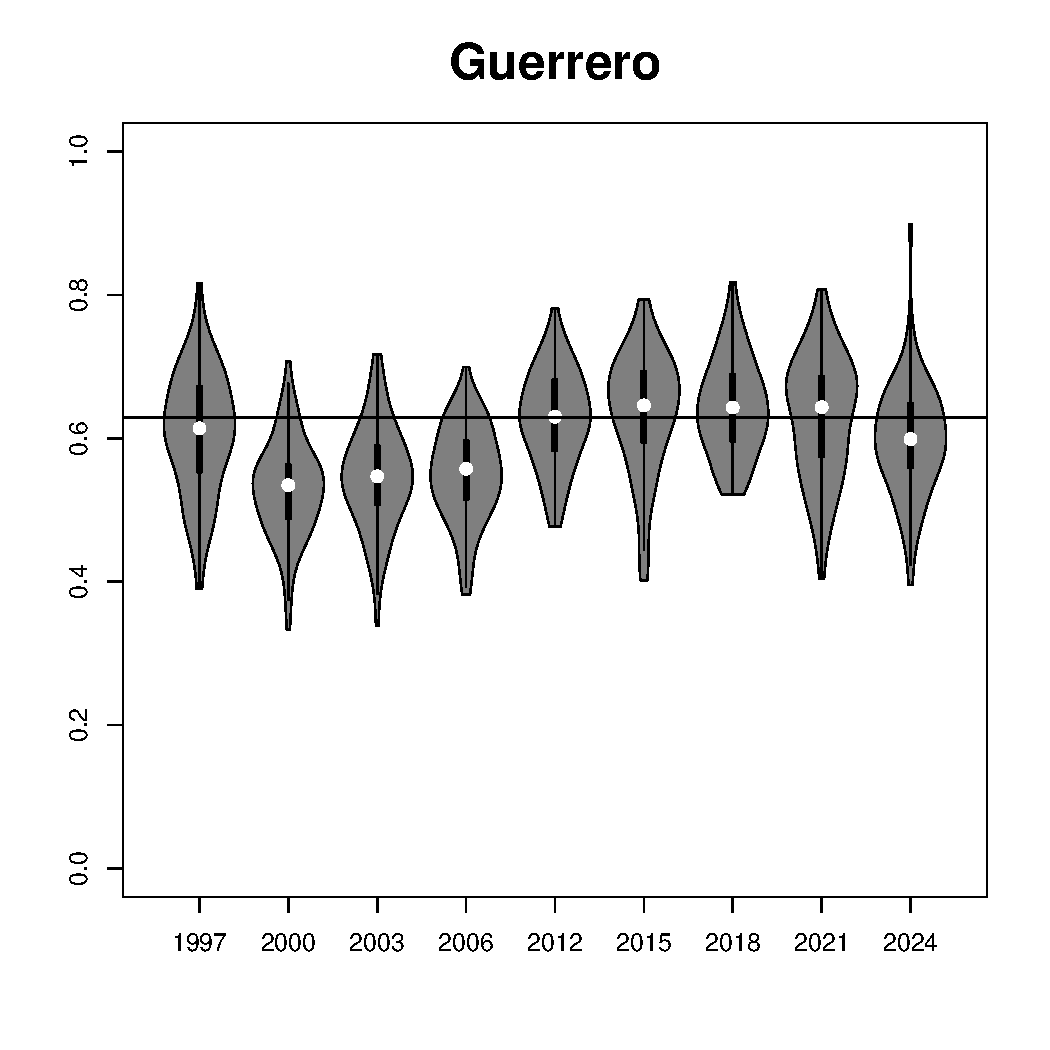
\includegraphics[width=.18\textwidth]{12.pdf} %&
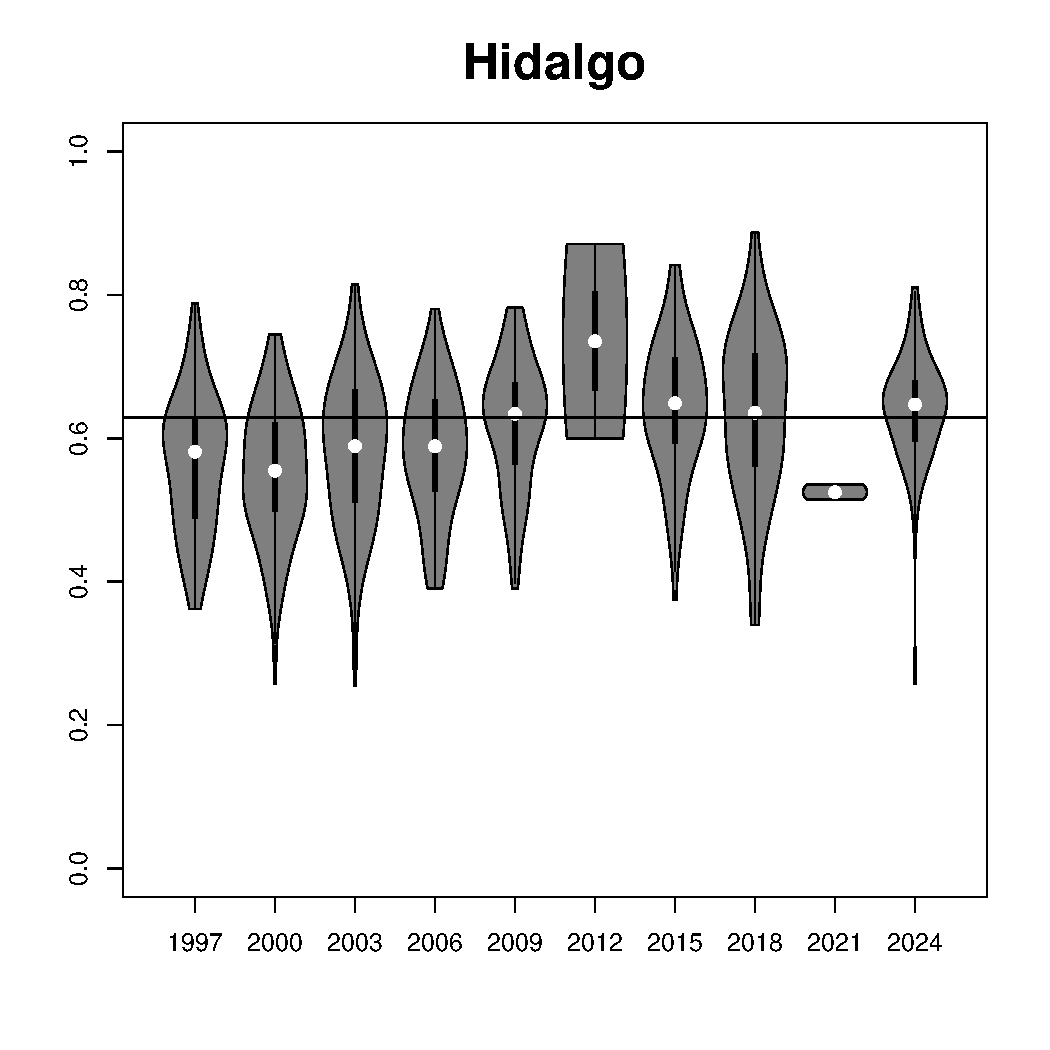
\includegraphics[width=.18\textwidth]{13.pdf} %&
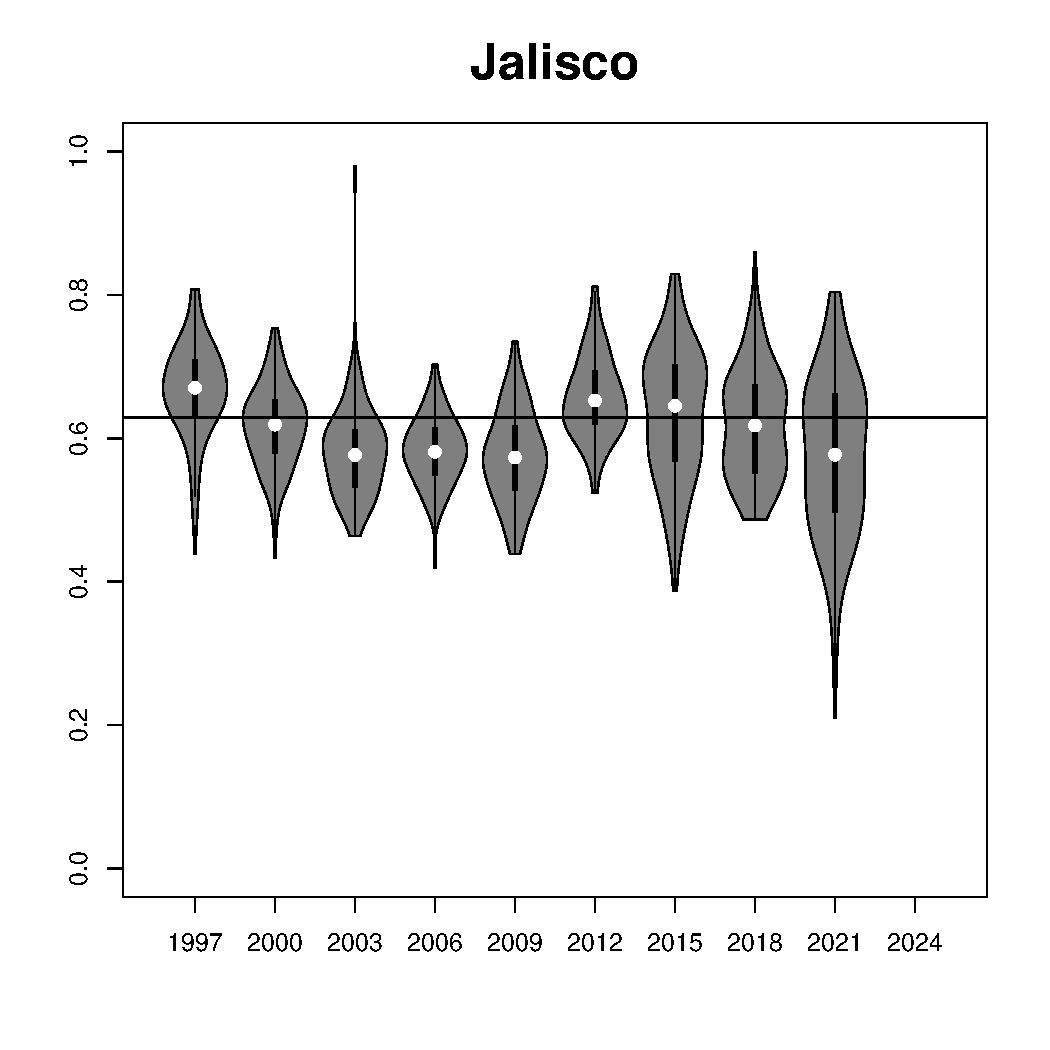
\includegraphics[width=.18\textwidth]{14.pdf} %&
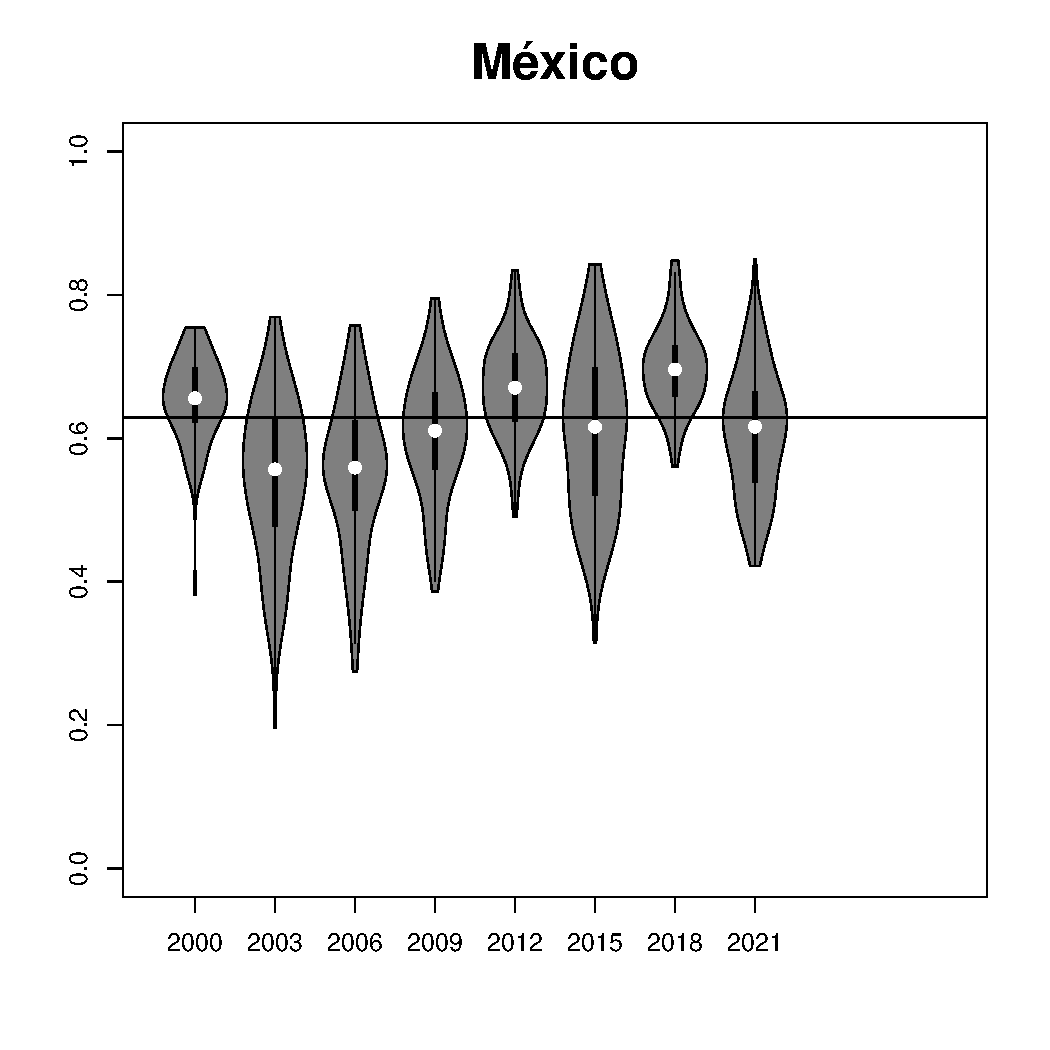
\includegraphics[width=.18\textwidth]{15.pdf} %\\
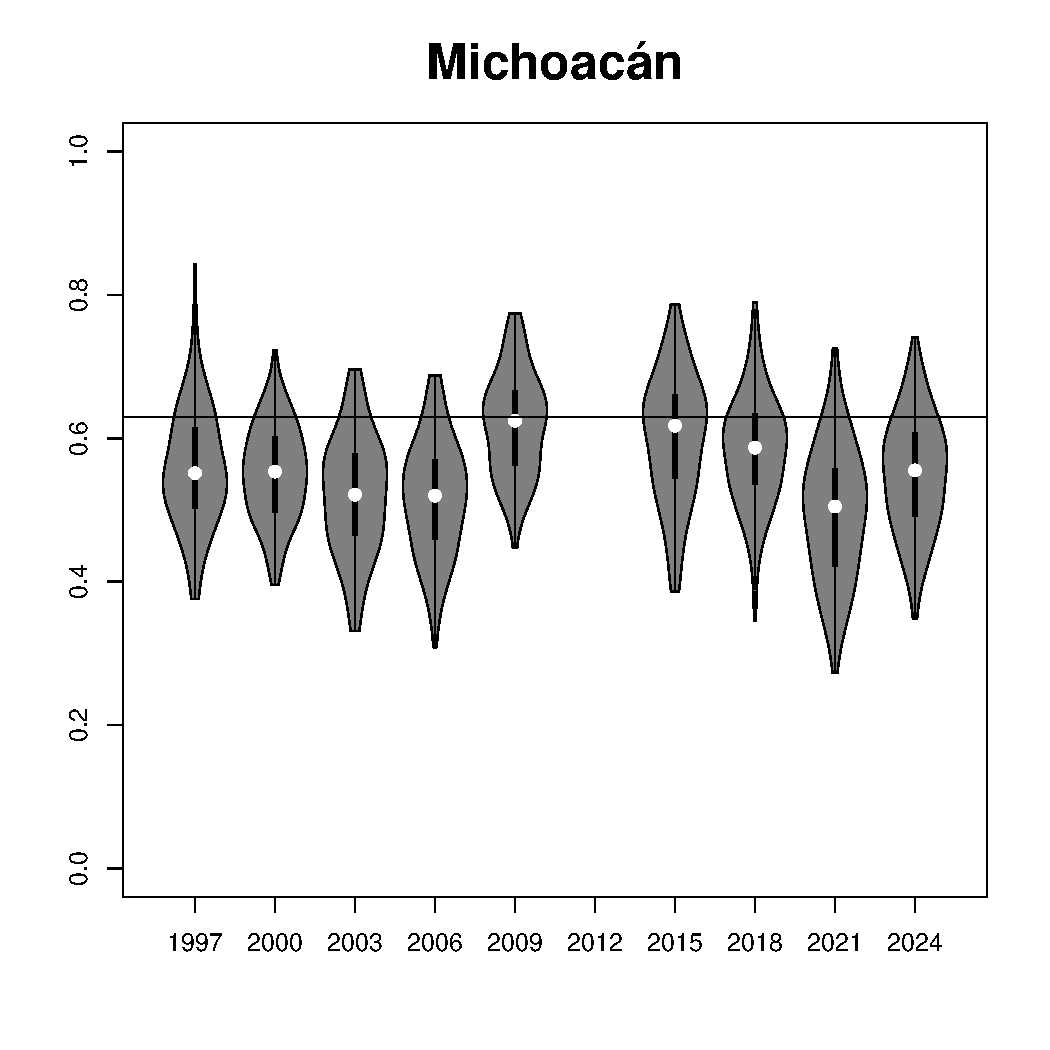
\includegraphics[width=.18\textwidth]{16.pdf} %&
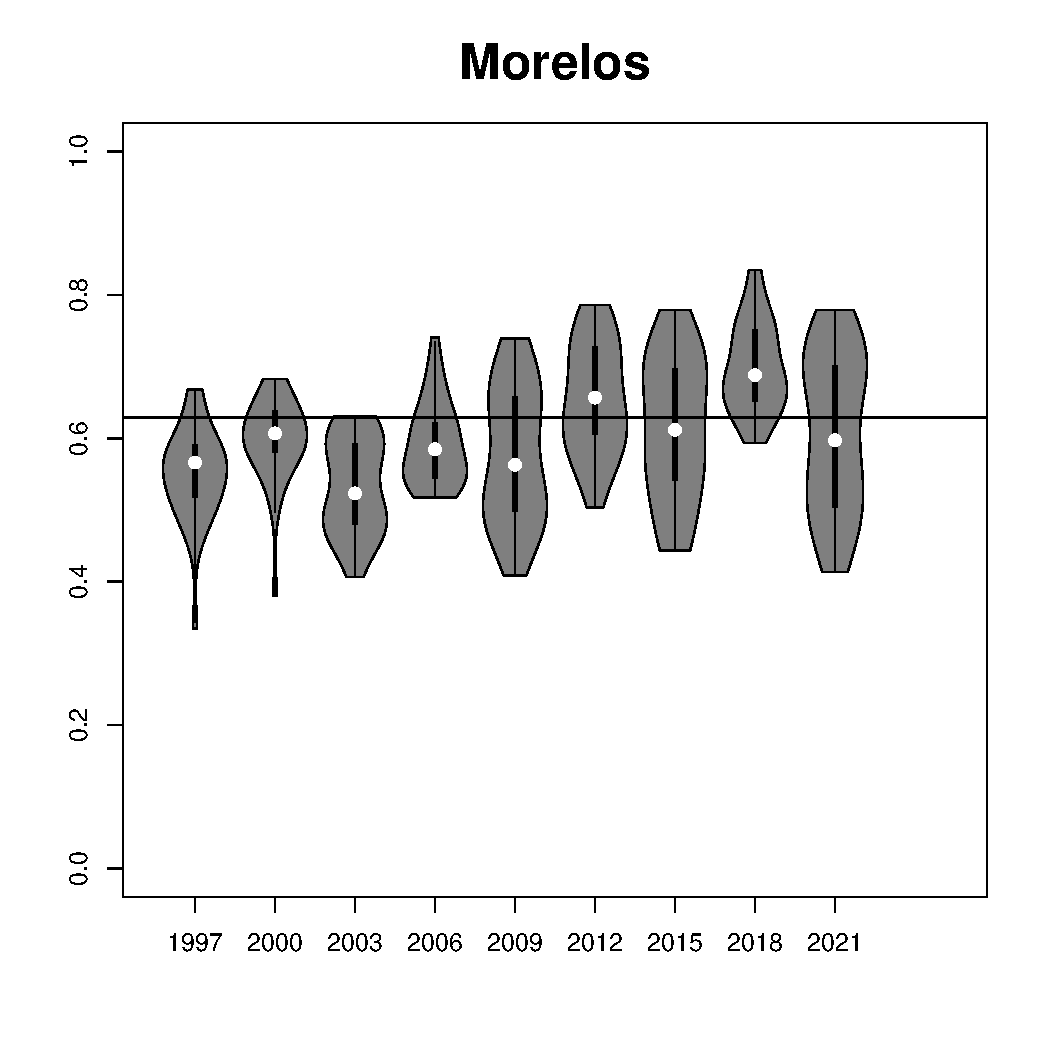
\includegraphics[width=.18\textwidth]{17.pdf} %&
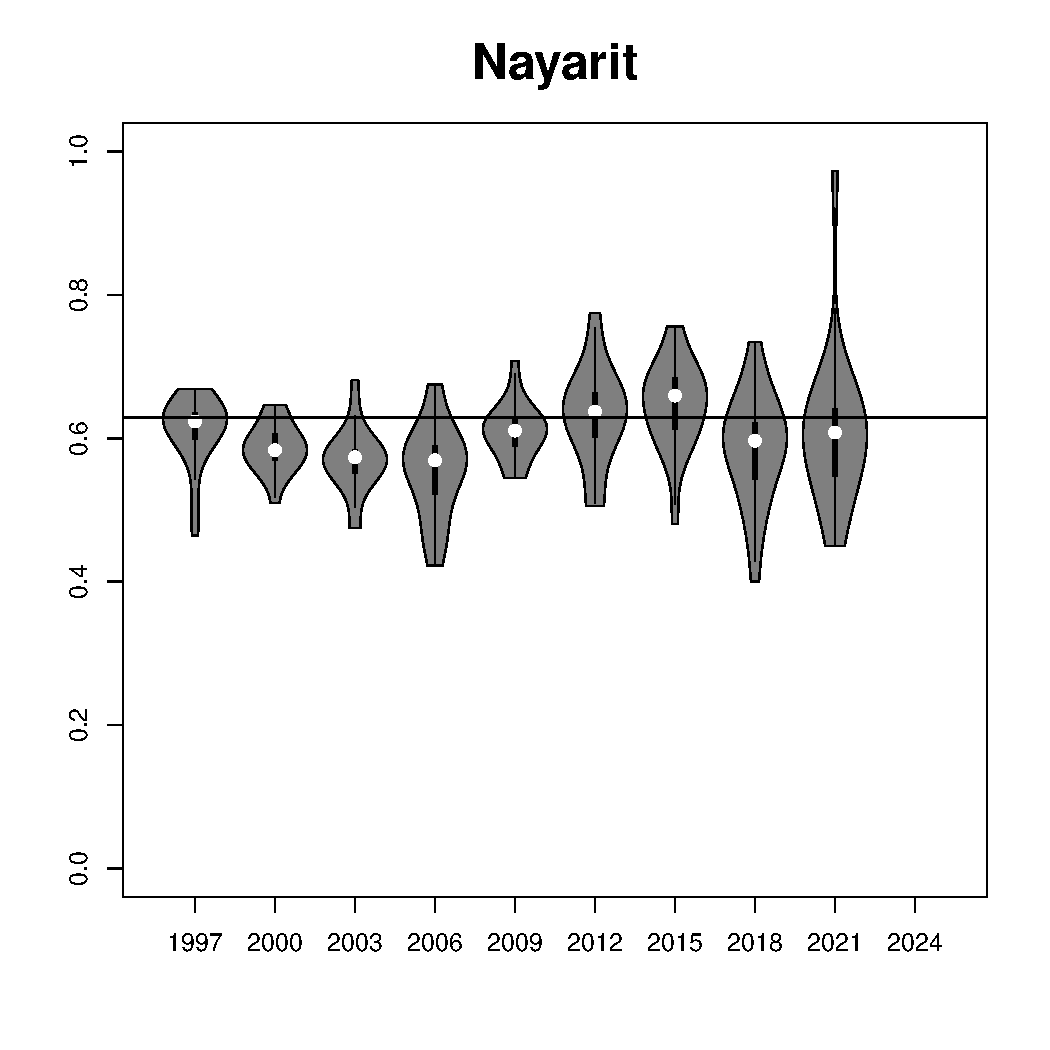
\includegraphics[width=.18\textwidth]{18.pdf} %&
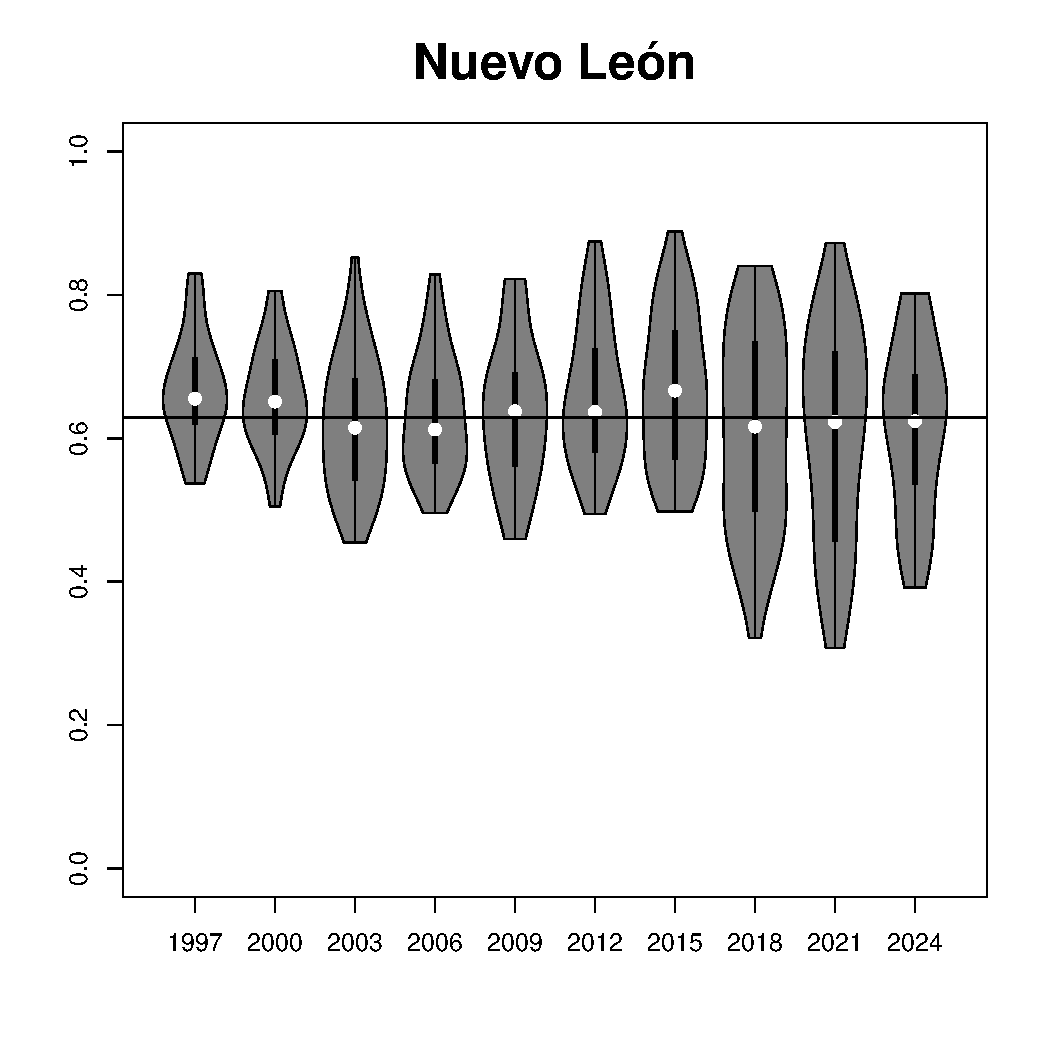
\includegraphics[width=.18\textwidth]{19.pdf} %&
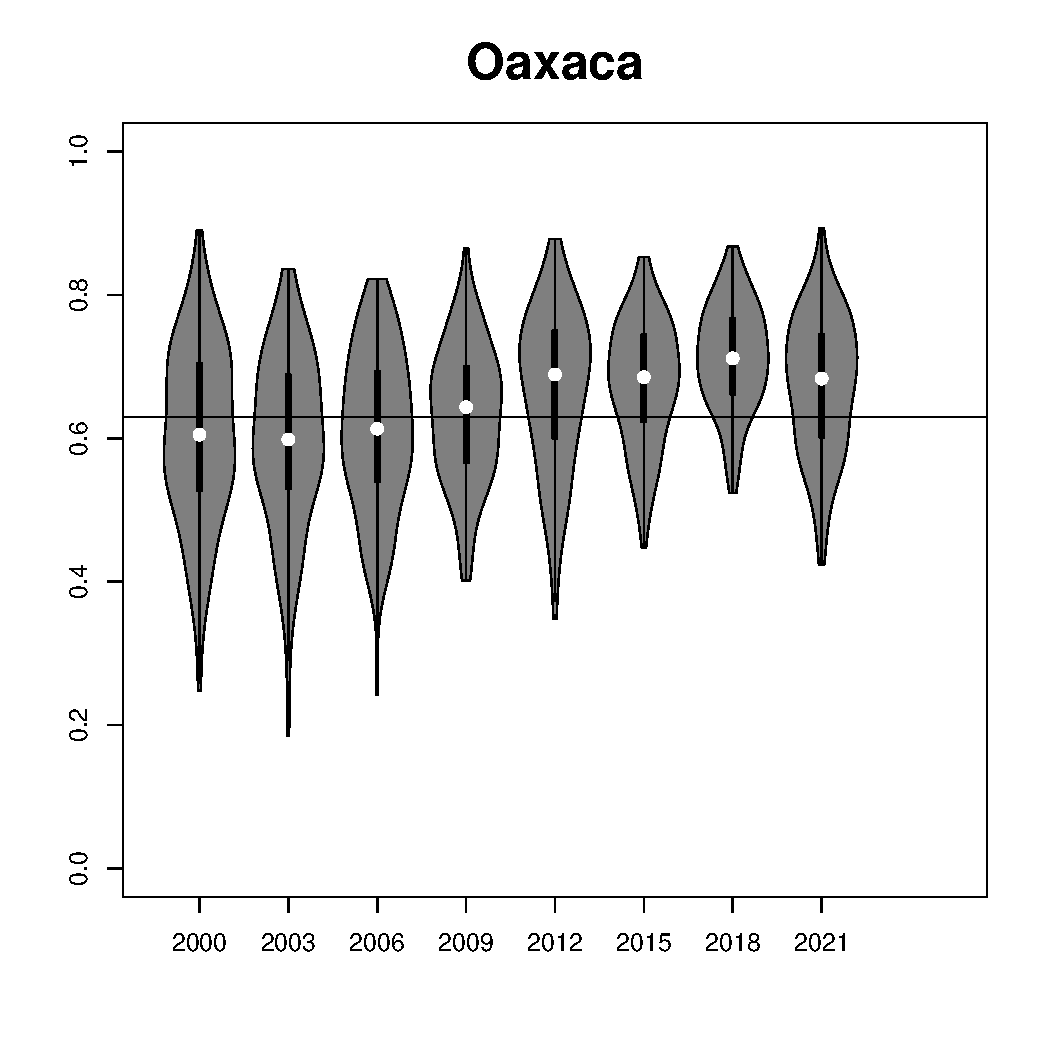
\includegraphics[width=.18\textwidth]{20.pdf} %\\
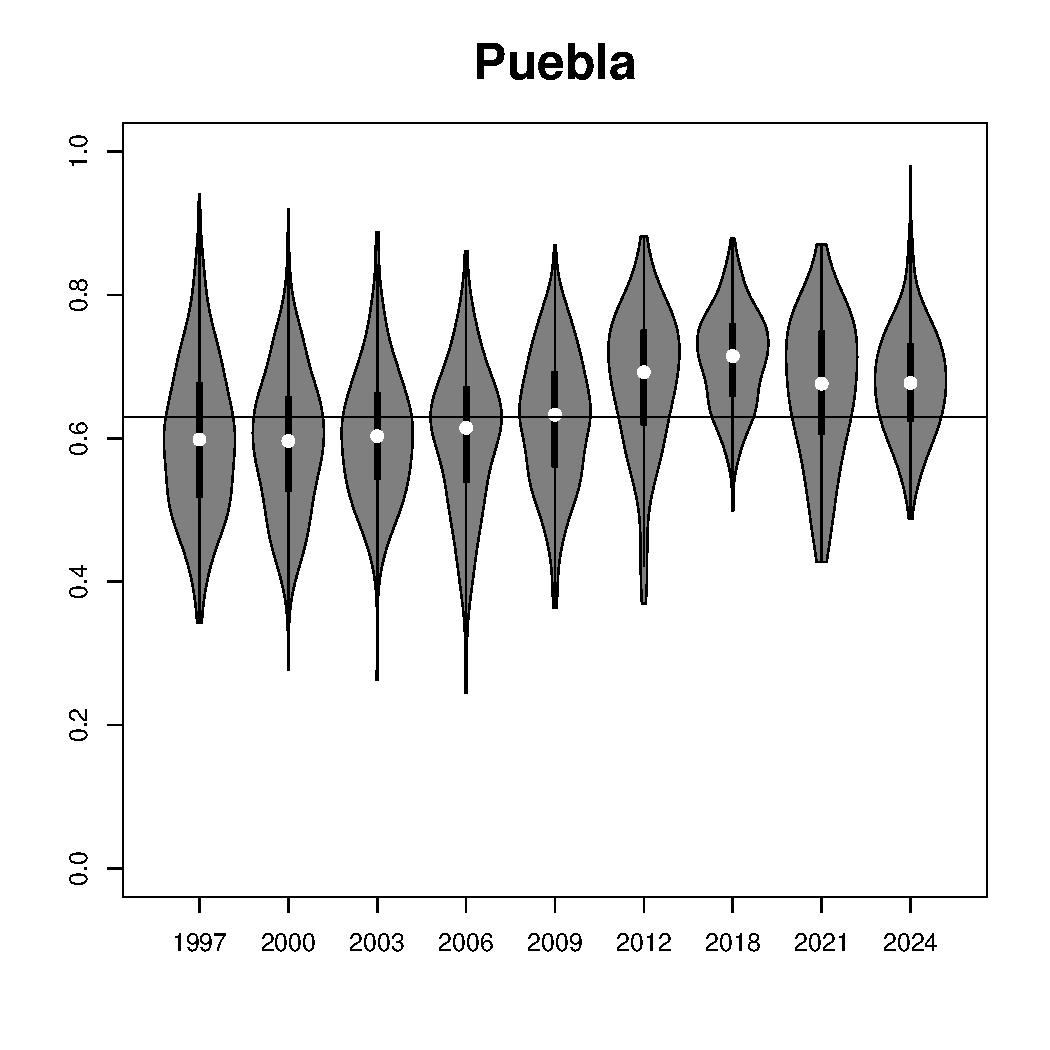
\includegraphics[width=.18\textwidth]{21.pdf} %&
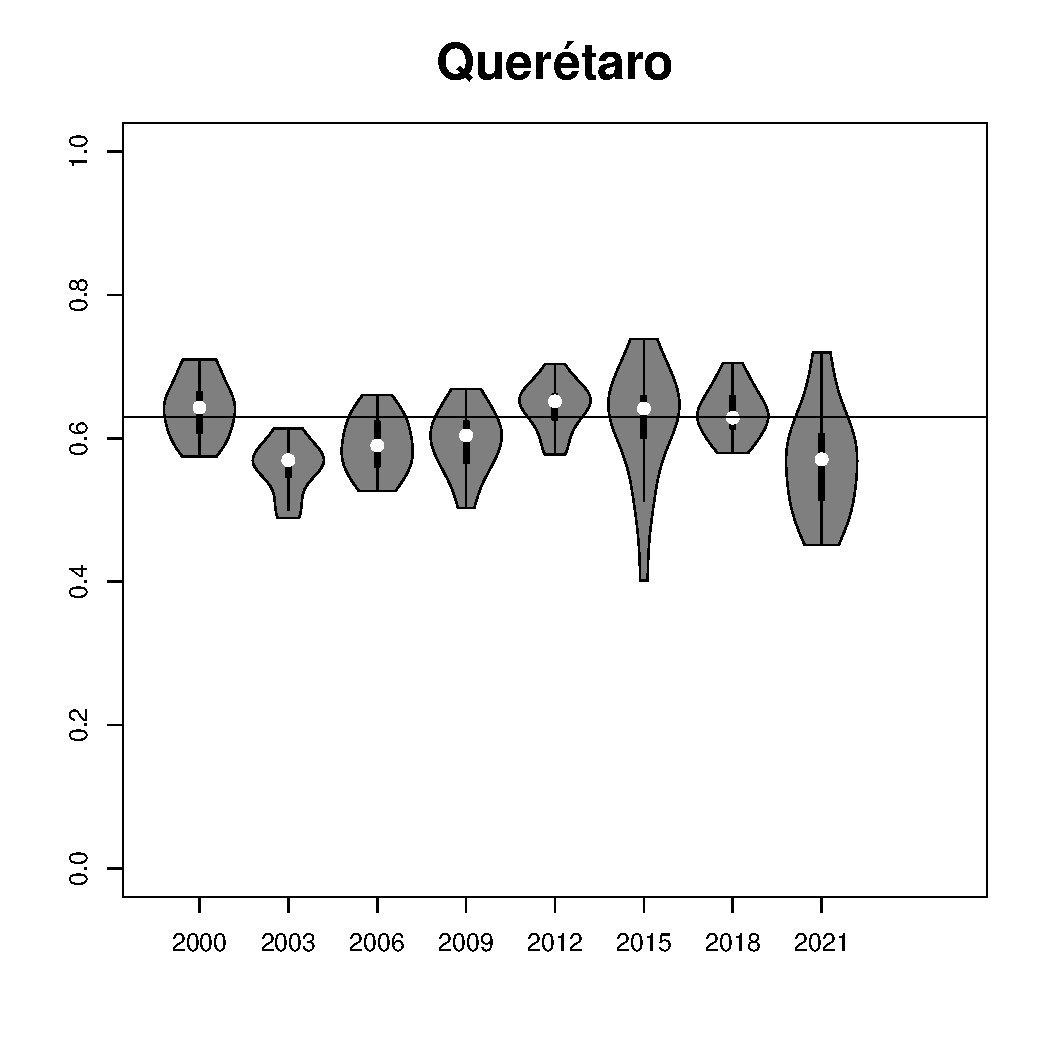
\includegraphics[width=.18\textwidth]{22.pdf} %&
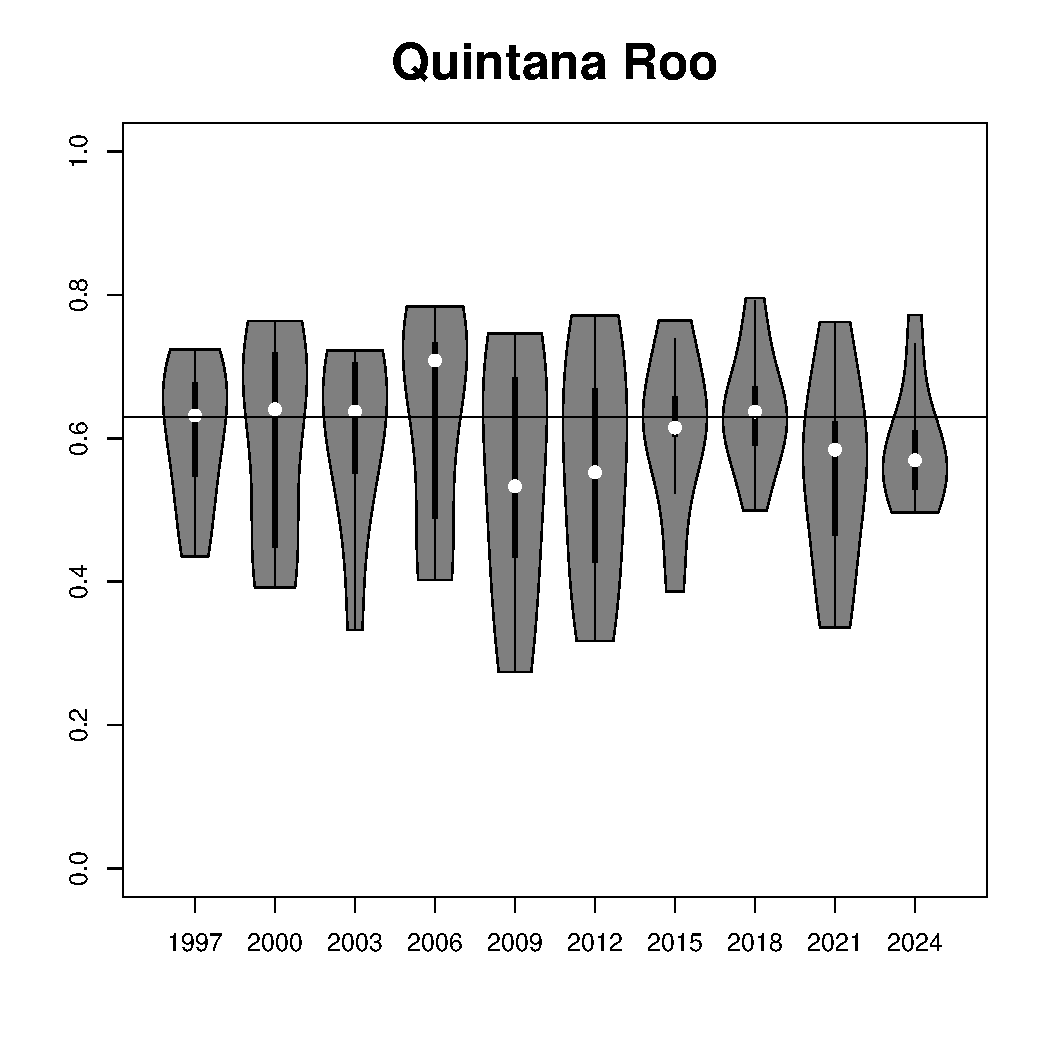
\includegraphics[width=.18\textwidth]{23.pdf} %&
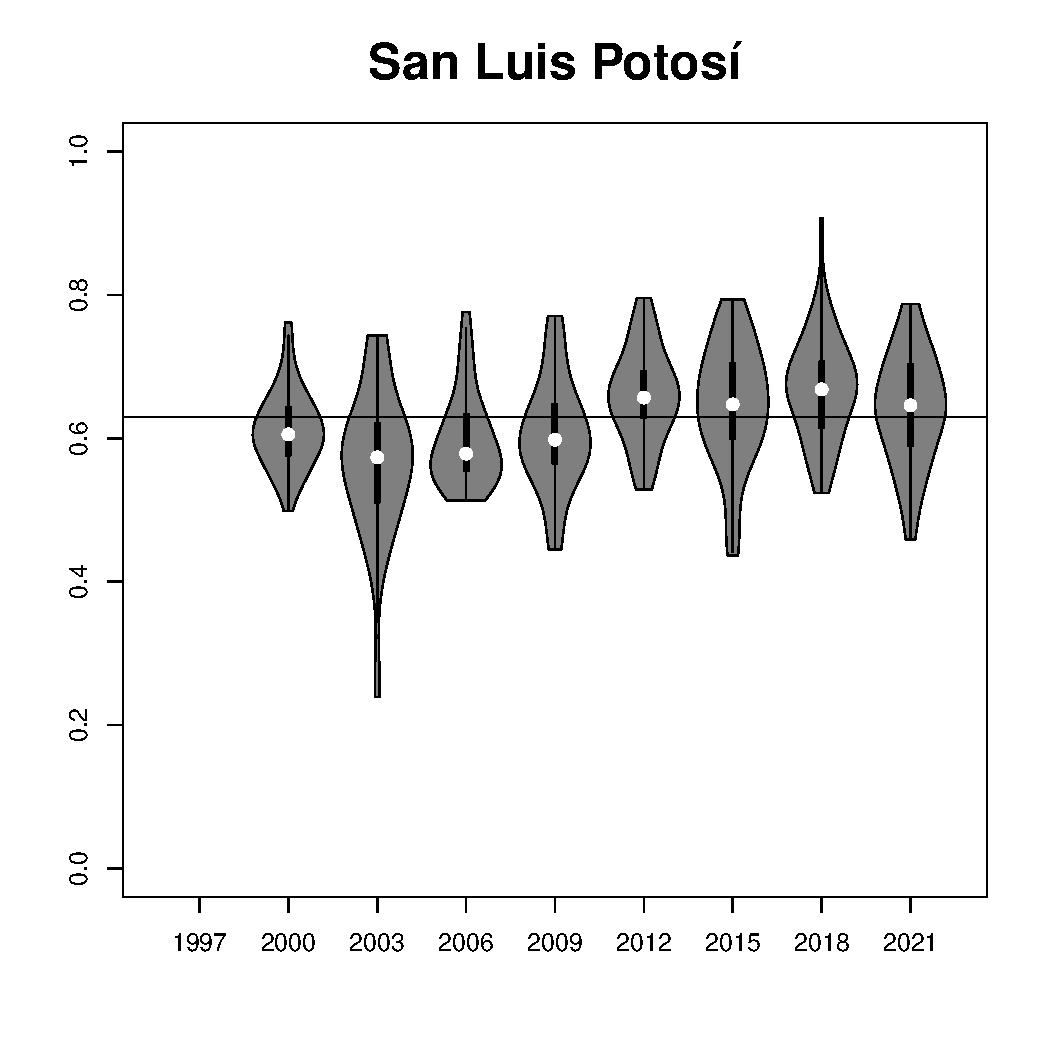
\includegraphics[width=.18\textwidth]{24.pdf} %&
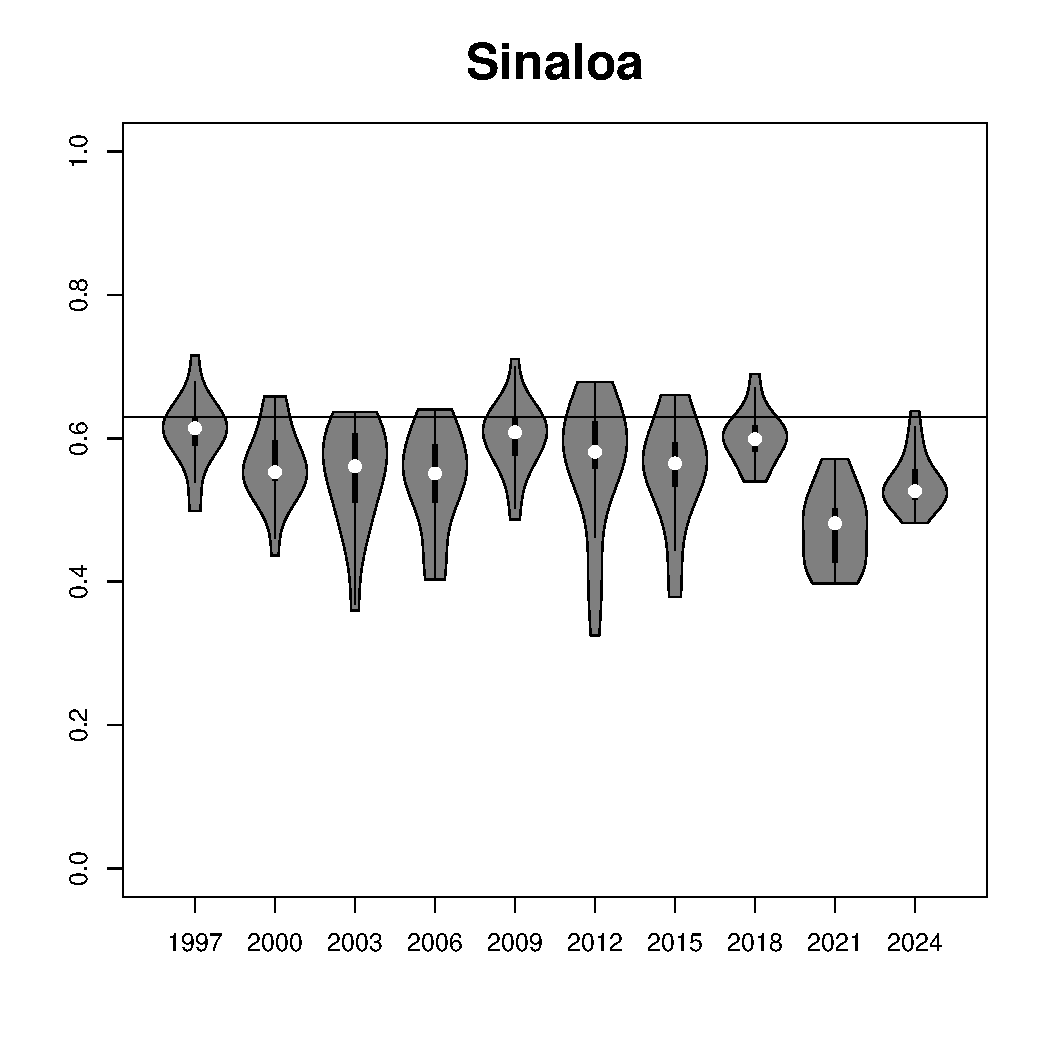
\includegraphics[width=.18\textwidth]{25.pdf} %\\
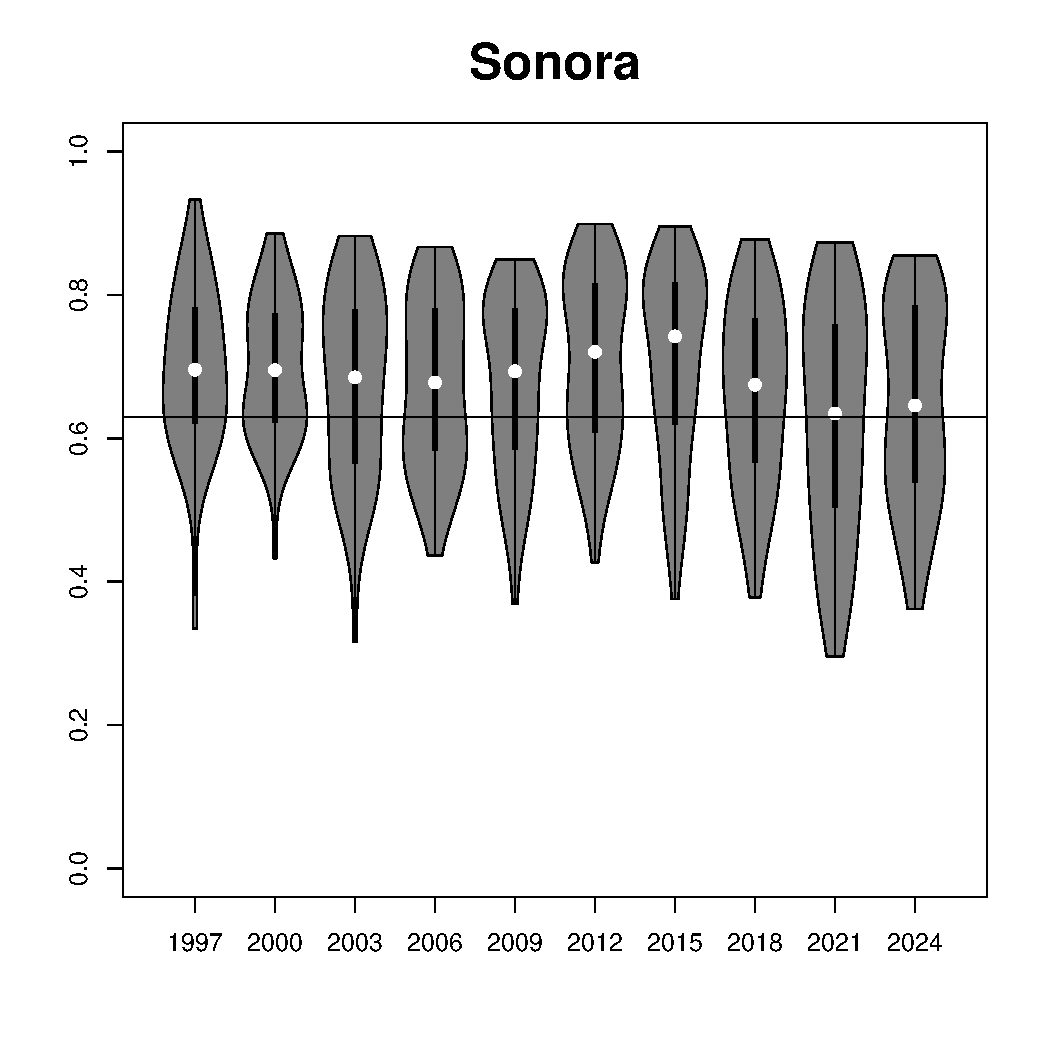
\includegraphics[width=.18\textwidth]{26.pdf} %&
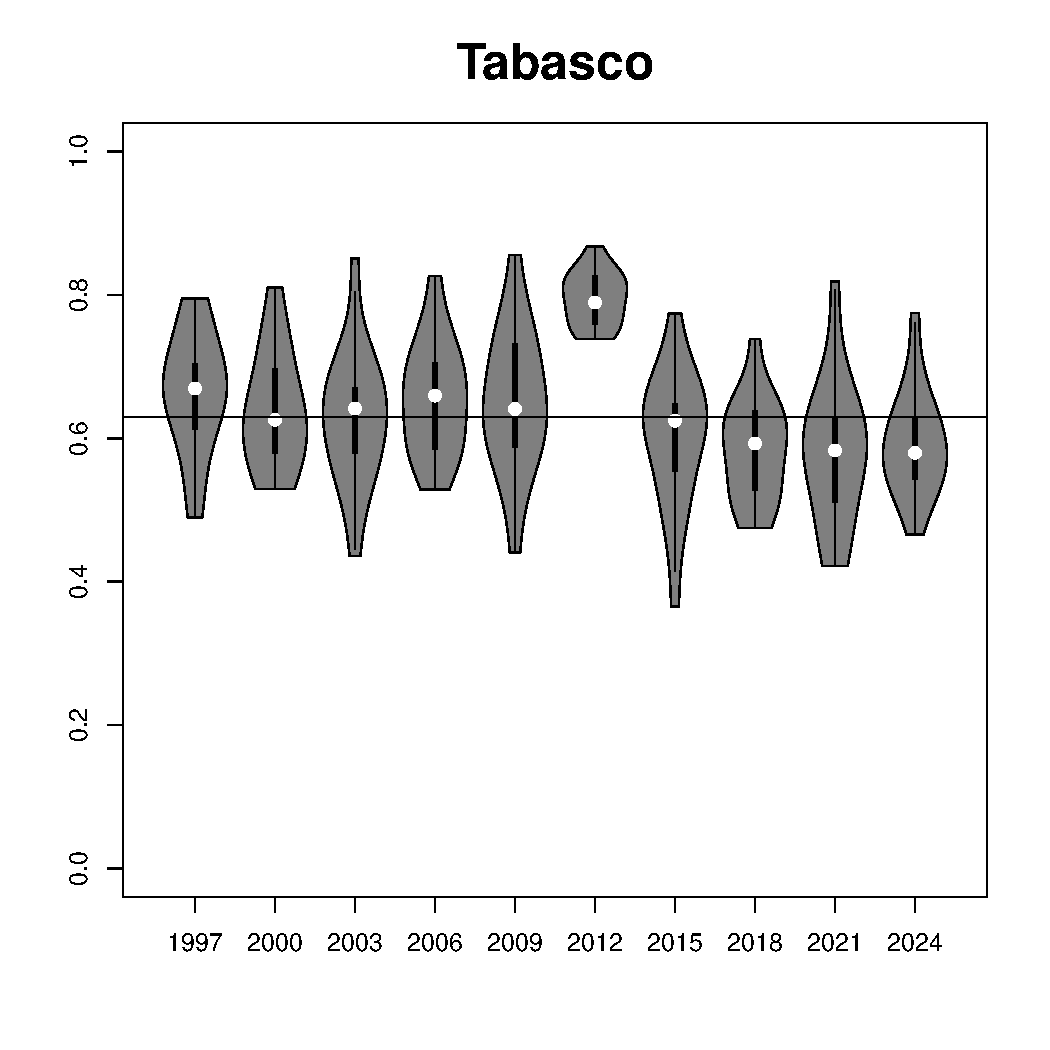
\includegraphics[width=.18\textwidth]{27.pdf} %&
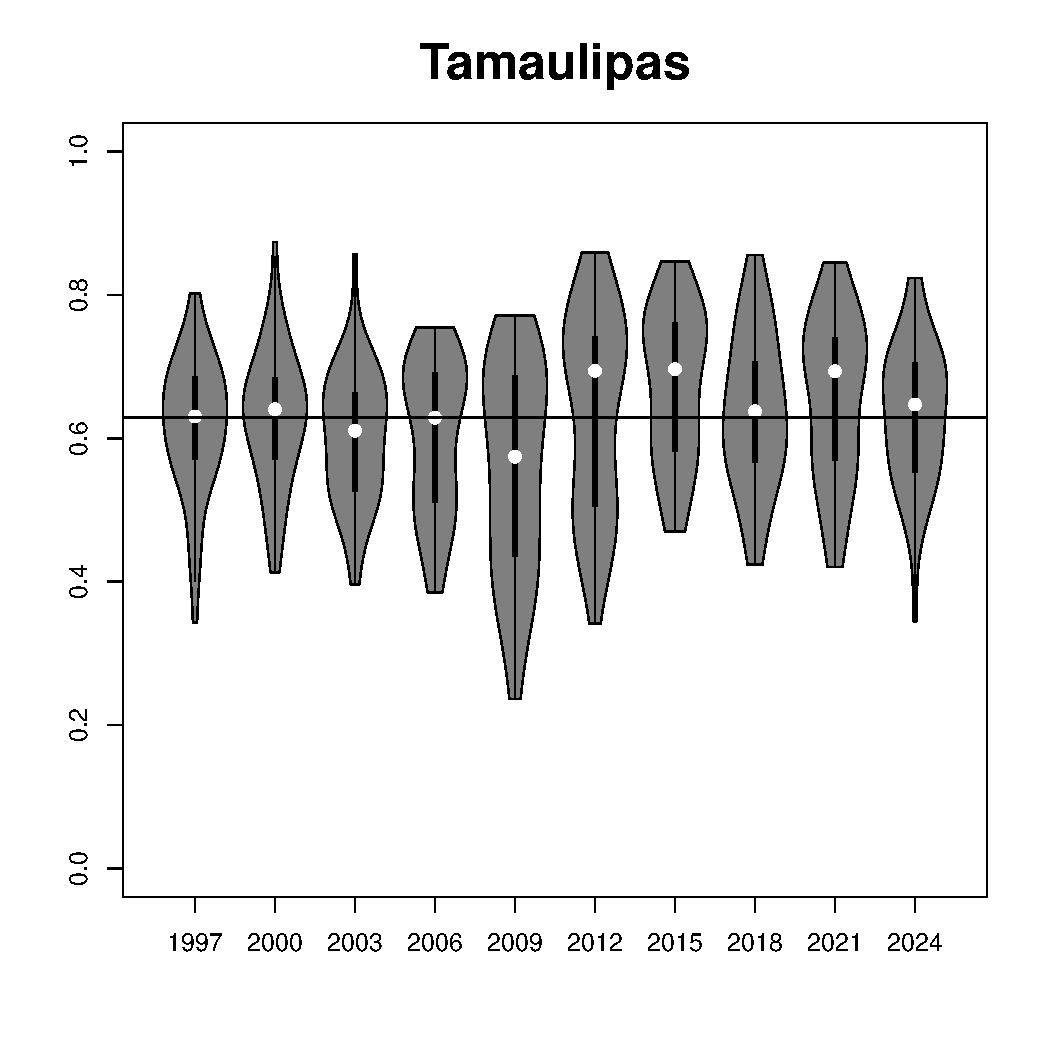
\includegraphics[width=.18\textwidth]{28.pdf} %&
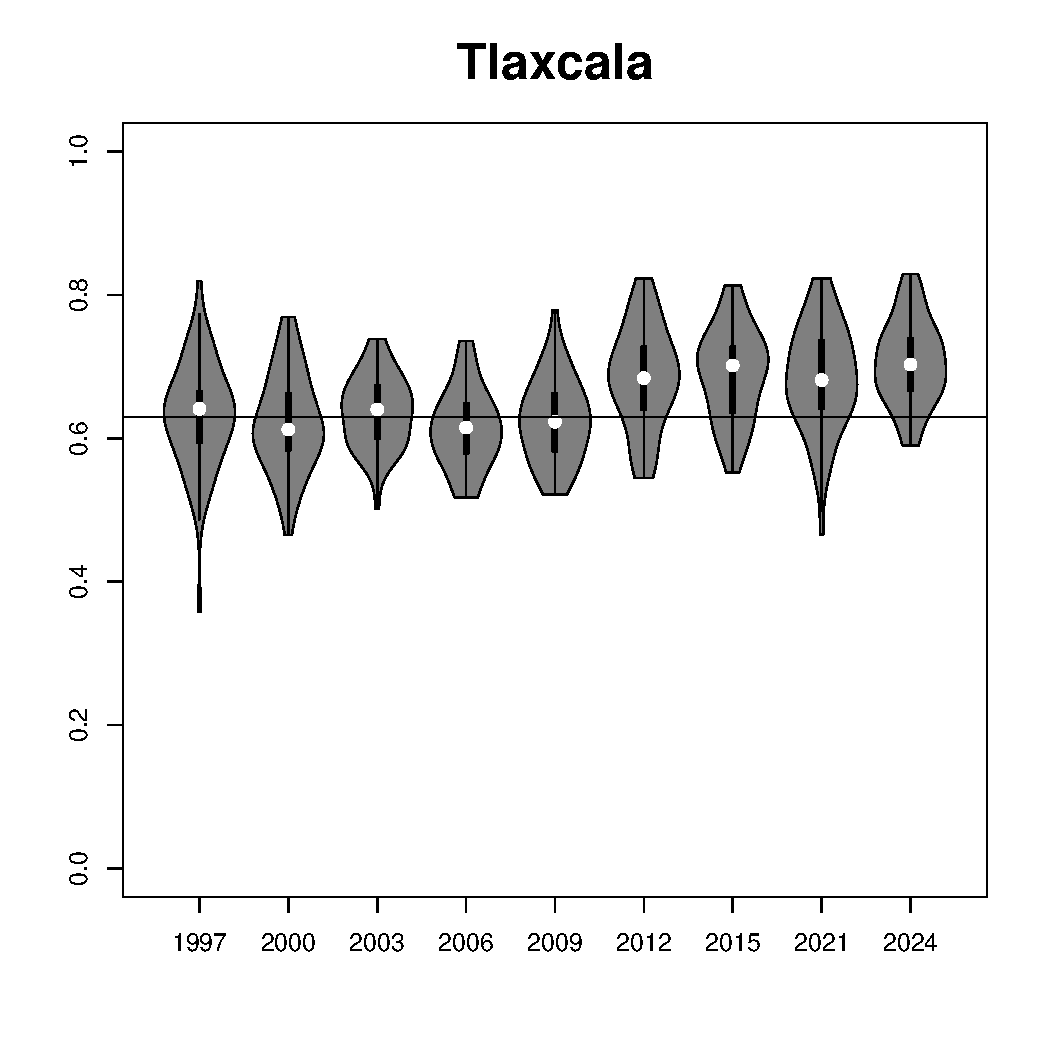
\includegraphics[width=.18\textwidth]{29.pdf} %&
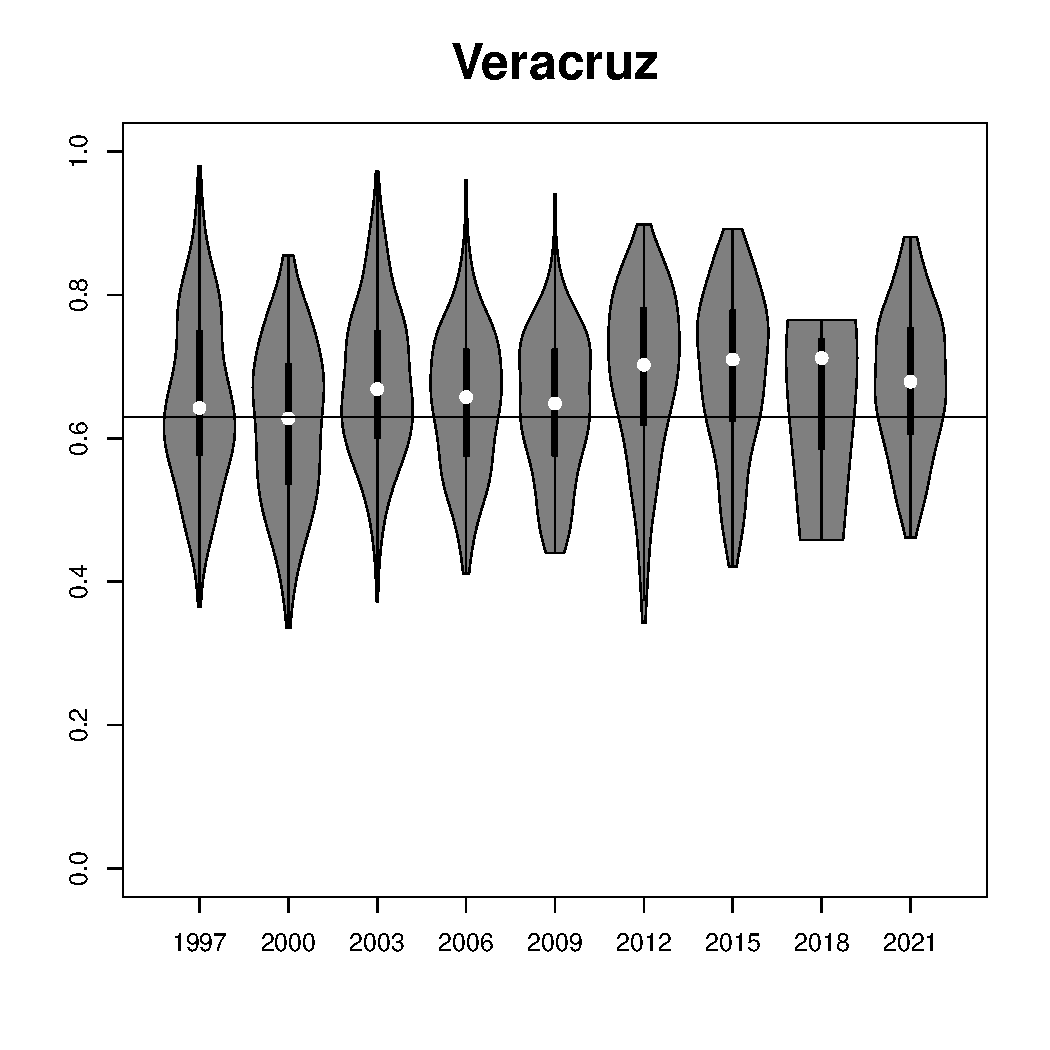
\includegraphics[width=.18\textwidth]{30.pdf} %\\
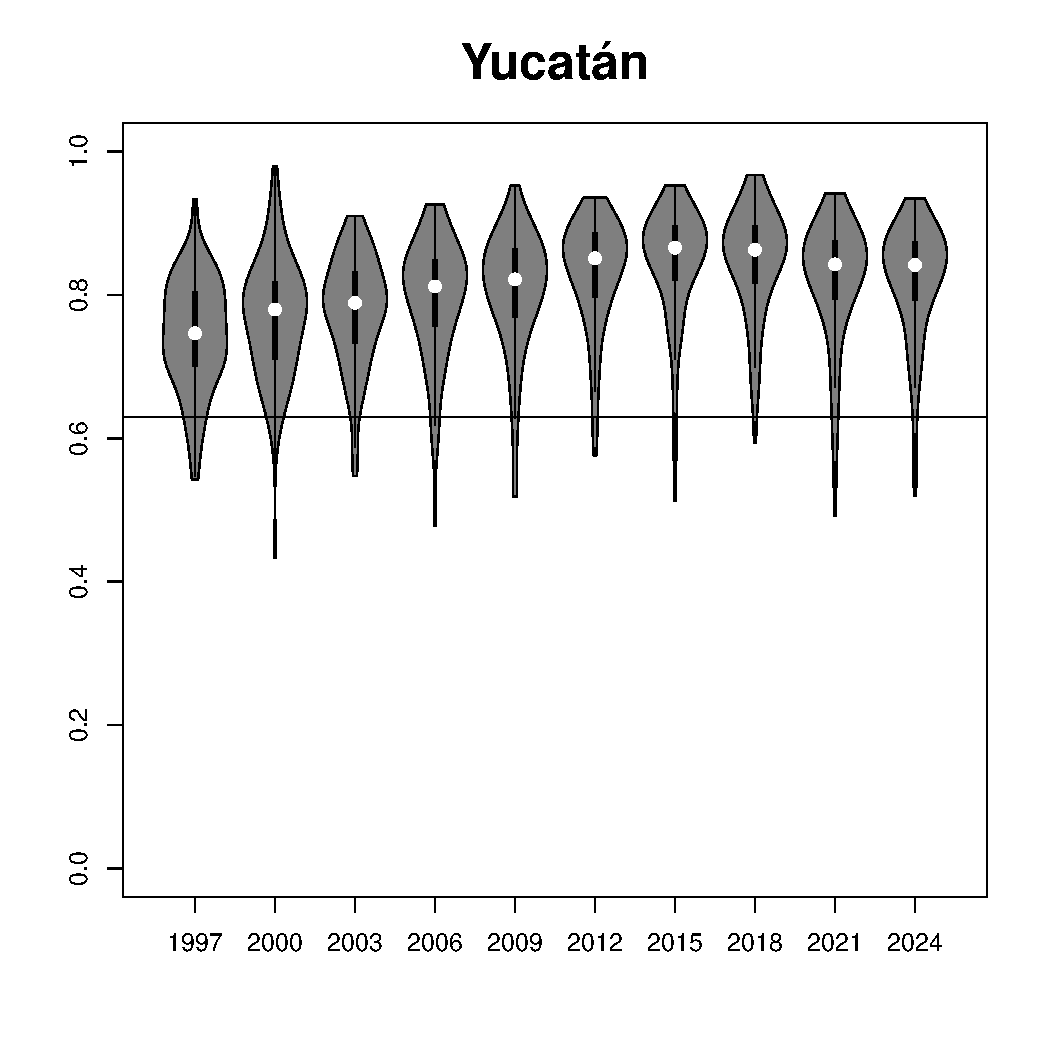
\includegraphics[width=.18\textwidth]{31.pdf} %&
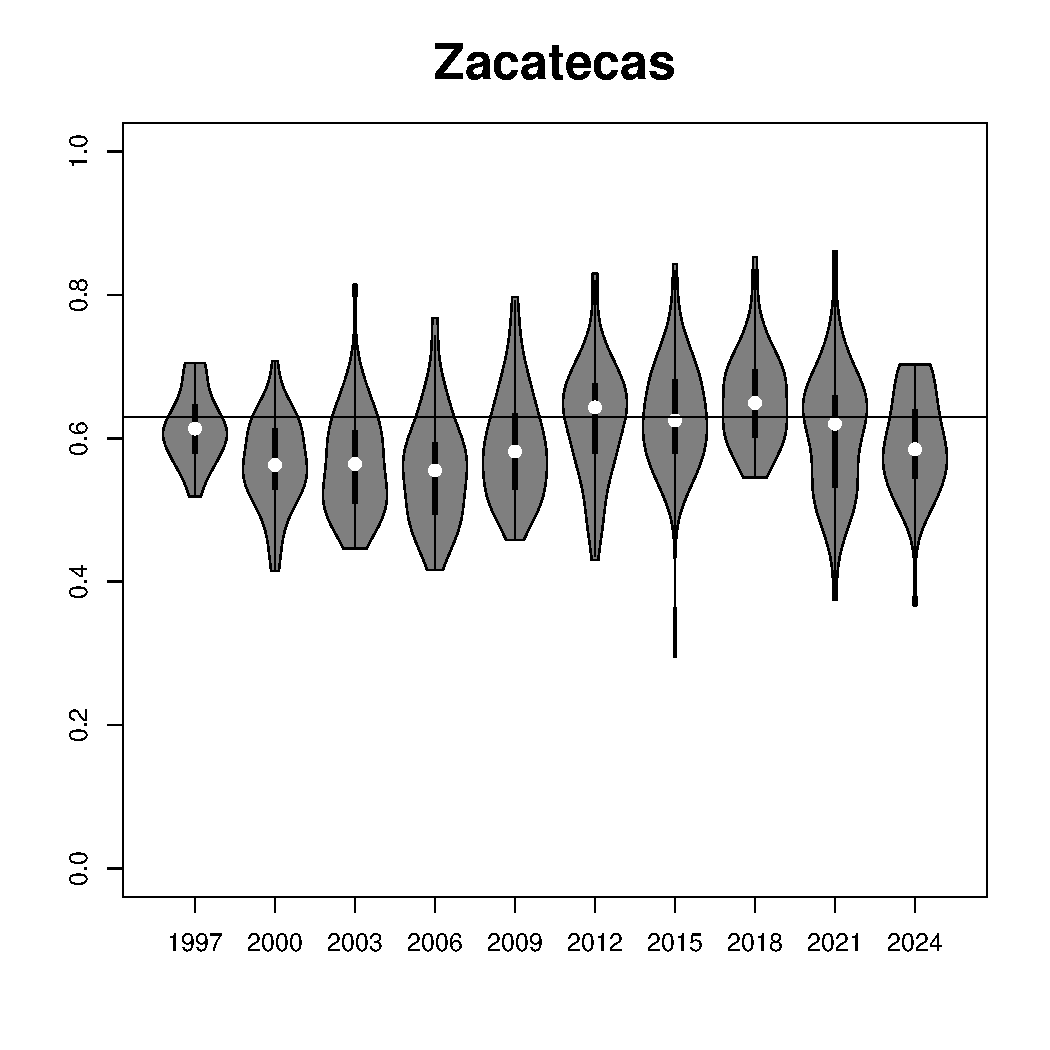
\includegraphics[width=.18\textwidth]{32.pdf} \\
% \end{tabular}

\end{document}


